%%%%%%%% ICML 2026 EXAMPLE LATEX SUBMISSION FILE %%%%%%%%%%%%%%%%%

\documentclass{article}

% Recommended, but optional, packages for figures and better typesetting:
\usepackage{microtype}
\usepackage{graphicx}
\usepackage{subcaption}
\usepackage{booktabs} % for professional tables

% hyperref makes hyperlinks in the resulting PDF.
% If your build breaks (sometimes temporarily if a hyperlink spans a page)
% please comment out the following usepackage line and replace
% \usepackage{icml2026} with \usepackage[nohyperref]{icml2026} above.
\usepackage{hyperref}


% Attempt to make hyperref and algorithmic work together better:
\newcommand{\theHalgorithm}{\arabic{algorithm}}

% Use the following line for the initial blind version submitted for review:
%\usepackage{icml2026}

% For preprint, use
%\usepackage{icml2026}

% If accepted, instead use the following line for the camera-ready submission:
\usepackage[accepted]{icml2026}

\usepackage{amsmath}
\usepackage{amssymb}
\usepackage{mathtools}
\usepackage{amsthm}
\usepackage{siunitx}



% if you use cleveref..
\usepackage[capitalize,noabbrev]{cleveref}

%%%%%%%%%%%%%%%%%%%%%%%%%%%%%%%%
% THEOREMS
%%%%%%%%%%%%%%%%%%%%%%%%%%%%%%%%
\theoremstyle{plain}
\newtheorem{theorem}{Theorem}[section]
\newtheorem{proposition}[theorem]{Proposition}
\newtheorem{lemma}[theorem]{Lemma}
\newtheorem{corollary}[theorem]{Corollary}
\theoremstyle{definition}
\newtheorem{definition}[theorem]{Definition}
\newtheorem{assumption}[theorem]{Assumption}
\theoremstyle{remark}
\newtheorem{remark}[theorem]{Remark}
\newtheorem{example}[theorem]{Example}

\usepackage{comment}
\usepackage{bbm}
\usepackage{algorithm}          % Algorithm float environment
\input{math_commands}
\usepackage{thmtools}
\usepackage{thm-restate}
\usepackage{enumitem}


%%%%%%%%%%%%%%%%%%%%%%%%%%%%%%%%
% CUSTOM MACROS
%%%%%%%%%%%%%%%%%%%%%%%%%%%%%%%%
\newcommand{\domain}{\mathcal{X}}
\newcommand{\codomain}{\mathcal{Y}}
\renewcommand{\epsilon}{\varepsilon}
\newcommand{\dd}{\mathrm{d}}

% Todonotes is useful during development; simply uncomment the next line
%    and comment out the line below the next line to turn off comments
%\usepackage[disable,textsize=tiny]{todonotes}
\usepackage[textsize=tiny]{todonotes}

% The \icmltitle you define below is probably too long as a header.
% Therefore, a short form for the running title is supplied here:
\icmltitlerunning{Sampling-Free Privacy Accounting for Matrix Mechanisms under Random Allocation}

\begin{document}
\addtolength{\dbltextfloatsep}{-1pt}
\addtolength{\dblfloatsep}{-1pt}
\addtolength{\intextsep}{-1pt}
\addtolength{\abovedisplayskip}{-.1\baselineskip}
\addtolength{\belowdisplayskip}{-.1\baselineskip}


\twocolumn[
  \icmltitle{Sampling-Free Privacy Accounting for Matrix Mechanisms\\ under Random Allocation}

  % It is OKAY to include author information, even for blind submissions: the
  % style file will automatically remove it for you unless you've provided
  % the [accepted] option to the icml2026 package.

  % List of affiliations: The first argument should be a (short) identifier you
  % will use later to specify author affiliations Academic affiliations
  % should list Department, University, City, Region, Country Industry
  % affiliations should list Company, City, Region, Country

  % You can specify symbols, otherwise they are numbered in order. Ideally, you
  % should not use this facility. Affiliations will be numbered in order of
  % appearance and this is the preferred way.
  \icmlsetsymbol{equal}{*}

  \begin{icmlauthorlist}
    \icmlauthor{Jan Schuchardt}{msmlr}
    \icmlauthor{Nikita Kalinin}{ista}
    \end{icmlauthorlist}

  \icmlaffiliation{msmlr}{Machine Learning Research, Morgan Stanley}
  \icmlaffiliation{ista}{Institute of Science and Technology Austria}
  
  \icmlcorrespondingauthor{Jan Schuchardt
}{jan.a.schuchardt@morganstanley.com}

  % You may provide any keywords that you find helpful for describing your
  % paper; these are used to populate the "keywords" metadata in the PDF but
  % will not be shown in the document
  \icmlkeywords{Machine Learning, ICML}

  \vskip 0.3in
]

% this must go after the closing bracket ] following \twocolumn[ ...

% This command actually creates the footnote in the first column listing the
% affiliations and the copyright notice. The command takes one argument, which
% is text to display at the start of the footnote. The \icmlEqualContribution
% command is standard text for equal contribution. Remove it (just {}) if you
% do not need this facility.

% Use ONE of the following lines. DO NOT remove the command.
% If you have no special notice, KEEP empty braces:
\printAffiliationsAndNotice{}  % no special notice (required even if empty)
% Or, if applicable, use the standard equal contribution text:
% \printAffiliationsAndNotice{\icmlEqualContribution}

\begin{abstract}
 We study privacy amplification for differentially private model training with matrix factorization under random allocation (also known as the balls-in-bins model). Recent work by Choquette-Choo et al. (2025) proposes a sampling-based Monte Carlo  approach to compute amplification parameters in this setting.
 However, their guarantees either only hold with some high probability or require random abstention by the mechanism.
 Furthermore, the required number of samples for ensuring $(\epsilon,\delta)$-DP is inversely proportional to $\delta$.
 In contrast, we develop sampling-free bounds based on Rényi divergence and conditional composition. 
 The former
 is facilitated by a dynamic programming formulation to efficiently compute the bounds. 
 The latter complements it by offering stronger privacy guarantees for small $\epsilon$, where R\'enyi divergence bounds inherently lead to an over-approximation.
 Our framework applies to arbitrary banded and non-banded matrices. Through numerical comparisons, we demonstrate the efficacy of our approach across a broad range of matrix mechanisms used in research and practice.
\end{abstract}

\section{Introduction}

Differential privacy (DP) \citep{dwork2006differential} offers one of the most well-established and mathematically rigorous definitions of privacy in statistical learning. In the context of deep learning, it is typically enforced via differentially private stochastic gradient descent (DP-SGD) \citep{abadi2016deep}. In DP-SGD, per-example gradients are clipped to bound the contribution of any individual data point, and Gaussian noise is added to guarantee privacy. While the injected noise inevitably degrades model utility, this loss can be mitigated through privacy \textit{amplification by subsampling}~\cite{li2012sampling}. Specifically, by randomly sampling a subset of the data at each iteration, we can achieve the same privacy guarantees with less additive noise. This improvement arises from the adversary’s uncertainty about which examples are included in each batch, introducing additional randomness that strengthens the overall privacy guarantees.

Several subsampling schemes have been studied in the context of differentially private training. One of the most commonly used is Poisson subsampling \citep{abadi2016deep, mironov2017renyi, koskela2020computing, zhu2022optimal}, in which each data point is independently included in a batch with a fixed probability chosen to achieve a desired expected batch size. However, this scheme poses practical challenges for implementation \citep{lebeda2025avoiding, beltran2024towards}. In particular, for large datasets and long training runs, two issues arise. First, drawing an independent random subset at every iteration is often computationally infeasible. Second, subsampling can lead to uneven data coverage, with a substantial fraction of examples (approximately $1/e$) not appearing within an epoch, and may increase the variance of gradients~\cite{feldman2025privacy}. As a result, a common but problematic practice is to train on shuffled data while reporting privacy guarantees derived for Poisson subsampling \citep{lebeda2025avoiding}.

A principled alternative that has emerged to address this issue is the  ``balls-in-bins'' scheme \citep{chua2024balls, choquette2024near}, also known as balanced iteration subsampling~\cite{dong2025leveraging} or as random allocation \citep{feldman2025privacy}. This approach predefines batches for an entire epoch and reuses them throughout training, ensuring a fixed number of participations per data point. As a result, it mitigates both the per-iteration sampling overhead and the uneven within-epoch data coverage, while requiring a noise multiplier comparable to that of Poisson subsampling to attain the same privacy guarantees. 

Beyond better subsampling schemes, another principled approach to improve upon the utility DP-SGD is to introduce correlated noise. The key idea is to add more noise at each iteration while carefully correlating it across steps so that the aggregate noise has lower variance than in standard DP-SGD, thereby improving model utility. The most common way to implement such noise correlations is through the matrix factorization mechanism \citep{li2015matrix, denisov2022improved, choquette2023multi, choquette-choo2023amplified}, where Gaussian noise $Z$ is correlated across iterations via the linear transformation $C^{-1}$, i.e., sampling $C^{-1}Z$, and then adding it to the gradients.
Matrix factorization, however, can be impractical at scale, motivating memory-efficient structured variants. Prior work proposes banded matrix factorizations~\citep{kalinin2024banded, mckenna2024scaling}, where the strategy matrix $C$ is banded and Toeplitz; banded-inverse factorizations~\citep{kalinin2025back}, where $C^{-1}$ is banded; and hybrid constructions such as the Buffered Linear Toeplitz (BLT) matrix~\citep{dvijotham2024efficient, mcmahan2024hassle}. These designs enable correlated-noise mechanisms with substantially reduced memory requirements.

Privacy amplification by subsampling and noise correlation techniques can be combined. This has been demonstrated for banded matrix mechanisms under Poisson subsampling \citep{choquette-choo2023amplified, choquette2023privacy}, and more recently for general correlation matrices using balls-in-bins subsampling \citep{choquette2024near}. The latter, however, relies on Monte Carlo estimation, which can require an intractably large number of samples in the high-privacy regime and thus become computationally expensive. Moreover, it does not directly yield deterministic DP guarantees, but rather privacy bounds that only hold with high probability.


Motivated by the recent independent works of \citet{feldman2025privacy,dong2025leveraging}, who derived privacy bounds for DP-SGD under balls-in-bins batching without Monte Carlo sampling, we propose two procedures for computing amplification bounds for matrix mechanisms under this batching scheme. Our methods avoid Monte Carlo sampling entirely and instead compute the bounds explicitly, leveraging R\'enyi divergence via dynamic programming
as well as conditional composition while accounting for the inter-step correlations unique to matrix mechanisms.


\textbf{Contribution}
\begin{itemize}[nosep]
    \item We introduce deterministic, Rényi divergence based and conditional composition based privacy analyses (accountants) for subsampled matrix mechanisms.
    %\item Our privacy accountants apply to arbitrary banded and non-banded matrices.
    \item For the special case of DP-SGD, we improve the computational complexity of R\'enyi accounting under the random allocation (balls-in-bins) batching scheme.
\end{itemize}


\section{Background}

\subsection{Definitions of Differential Privacy}\label{section:privacy_definitions}

\textit{Differential Privacy (DP)}  is a widely accepted framework for providing rigorous privacy guarantees. We recall its definition below:


\begin{definition}[Differential Privacy \citep{dwork2006differential}]
A randomized mechanism is said to provide $(\varepsilon, \delta)$-differential privacy under a neighboring relation $\simeq$ if, for all datasets $D \simeq D'$, and for all measurable subsets $S$ of the mechanism's output space:
\begin{equation}
\Pr[M(D) \in S] \leq e^{\varepsilon} \cdot \Pr[M(D') \in S] + \delta.
\end{equation}
\end{definition}
In the following, we  write $M(\cdot \mid D)$ for the distribution of random variable $M(D)$.
We further use 
an equivalent definition of differential privacy that is more convenient for privacy accounting, i.e., tracking privacy over multiple applications of a mechanism.
\begin{lemma}[Proposition 2 from~\cite{barthe2013beyond}]
    A mechanism provides $(\epsilon, \delta)$-DP under $\simeq$ if and only if, for all $D \simeq D'$,
    $
        H_{e^\epsilon}\left(M(\cdot \mid D), M(\cdot \mid D')\right) \leq \delta
    $
    with hockey-stick divergence
    \begin{equation}\label{definition:hockey_stick_divergence}
        H_{\gamma}(P|| Q) = \mathbb{E}_{x \sim P} \left[ \max\left\{ 1 - \gamma \frac{\dd Q}{\dd P}(x),\; 0 \right\} \right].
    \end{equation}
\end{lemma}
While $(\epsilon,\delta)$-DP corresponds to a bound on the hockey-stick divergence for a single choice of 
$\gamma=e^\epsilon$, tight privacy accounting requires bounds for all choices of $\gamma$.
In the following, we recall multiple equivalent~\cite{zhu2022optimal} characterizations of this~\emph{privacy profile} that are immediately relevant to  our work, beginning with dominating pairs:
\begin{definition}
    We say that the pair of distributions $(\hat{P}, \hat{Q})$ dominates $(P,Q)$, denoted by $(P,Q) \prec (\hat{P},\hat{Q})$, 
    if $H_\gamma(P||Q) \leq H_\gamma(\hat{P},\hat{Q})$ for all $\gamma > 0$.
\end{definition}
\begin{definition}[\citet{zhu2022optimal}]
    We say that $(\hat{P}, \hat{Q})$ are a \emph{dominating pair} of mechanism $M$ under neighboring relation $\simeq$ if
    $(M(\cdot \mid D), M(\cdot \mid D')) \prec (\hat{P}, \hat{Q})$ for all $D \simeq D'$.
\end{definition}
Given a dominating pair $(P,Q)$, the problem of privacy accounting reduces to quantifying the hockey-stick divergence $H_\gamma(P||Q)$. Specifically, the divergence does not directly depend on the (potentially high-dimensional) structure of $(P, Q)$ but on their log-likelihood ratio, the ``privacy loss'':
\begin{definition}
    The privacy loss random variable $L_{P,Q}$ of two distributions $P,Q$ is $\log(\frac{\dd P}{\dd Q}(x))$ with $x \sim P$.
\end{definition}
From~\cref{definition:hockey_stick_divergence} and $\gamma \frac{\dd P}{\dd Q}(x) = e^{\log(\gamma) - L_{P,Q}}$, we see that the hockey-stick divergence quantifies  how much the privacy loss random variable exceeds $\epsilon=\log(\gamma)$ (in expectation).
While the density of $L_{P,Q}$ fully determines the privacy profile, it is often analytically more convenient to work with its moment-generating properties. Specifically, the privacy loss distribution 
is uniquely characterized by its cumulant generating function~\cite{zhu2022optimal}, which is proportional to the Rényi divergence:
\footnote{R\'enyi divergences of dominating pairs are not to be confused with R\'enyi DP~\cite{mironov2017renyi}, which is a strictly less informative notion of privacy, see Appendix A in~\cite{zhu2022optimal}.}
\begin{definition}
    The R\'enyi divergence of $P$ and $Q$ is
    \begin{equation}
        R_\alpha(P||Q) = \frac{1}{\alpha - 1} \log \mathbb{E}\left[  e^{ (\alpha - 1) L_{P,Q}} \right].
    \end{equation}
\end{definition}

\subsection{(Subsampled) Matrix Mechanisms}\label{section:background_matrix_mechanisms}

Training a private model with $d$ parameters using differentially private stochastic gradient descent (DP-SGD) for $k$ epochs with $b$ batches per epoch (and thus $N = k \cdot b$ iterations) can be viewed as sequentially computing the noisy prefix sums $\mathbf{E}(\mG + \mZ)$ row by row, where $\mathbf{E} \in \{0,1\}^{N \times N}$ is the all-ones lower-triangular matrix; the entries of $\mZ \in \sR^{N \times d}$ are drawn i.i.d.\ from a normal distribution with standard deviation $\sigma > 0$; and $\mG \in \sR^{N \times d}$ contains the aggregated gradients for each batch, clipped to a fixed $\ell_2$-norm.

%Other first-order optimizers (e.g., SGD with momentum) can similarly be expressed as $\mA \mG$ with a general \emph{workload matrix} $\mA \in \sR^{n \times n}$.
%Differentially private stochastic gradient descent (DP-SGD) approximates this prefix sum privately
%via $\mA \mG \approx \mA \overline{\mG} + \mZ$, where the gradients in $\mG$ are clipped before averaging to obtain $\overline{\mG}$ , and .

Over the past few years, various works have theoretically and empirically demonstrated that improved estimation can be achieved by correlating the noise across iterations. Specifically, by introducing a so-called correlation matrix $\mC^{-1} \in \sR^{N \times N}$, the matrix factorization mechanism \citep{li2015matrix} adds correlated noise via $\mathbf{E}\bigl(\mG + \mC^{-1}\mZ\bigr)$. This approach, however, requires adjustments to the privacy accounting. Without subsampling, it is equivalent (by the post-processing property) to applying the Gaussian mechanism to make $\mC\mG$ private by adding noise $\mZ$, and it therefore requires computing the corresponding sensitivity \citep{choquette-choo2023amplified}. The resulting scheme can offer superior utility: although the sensitivity may increase (and thus the noise scale must be adjusted accordingly), the total injected noise $\mathbf{E}\mC^{-1}\mZ$ can have a much smaller expected norm. By adding less noise to the intermediate models, training utility can improve; see the recent survey \citep{pillutla2025correlated} for further discussion on selecting a correlation matrix.


%are made possible by factorizing the workload matrix as $\mA = \mB \mC$ with invertible $\mB, \mC \in \sR^{n \times n}$.
%Concretely, the approximation
%$(\mB \mC) \mG
%\approx
%\mB (\mC \overline{\mG} + \mZ)
%=
%(\mB \mC) ( \overline{\mG} + \mC^{-1} \mZ)$ can result in much smaller expected errors. Put simply, this means that  correlated  noise with covariance $\mC^{-1} \mC^{-T}$ often offers superior utility at the same privacy level.

The utility of the matrix factorization mechanism can be further improved by combining it with amplification by subsampling. A recent work by \citet{choquette2024near} introduces an efficient balls-in-bins subsampling scheme, along with a corresponding privacy accountant that supports matrix factorization with an arbitrary positive lower-triangular \emph{strategy} matrix~$\mC$.


%Specifically, the privacy of these matrix mechanisms is determined by strategy matrix $\mC \in \sR^{n \times n}$, the ratio $\frac{\sigma}{\Delta}$ of standard deviation $\sigma$ and $\ell_2$ clipping norm $\Delta$, as well as the used~\emph{subsampling scheme}, i.e.,
%which training sample contributes to which of %the $n = k \cdot b$ batches.
%As previously discussed, our work focuses on the following subsampling scheme that is appealing from both an implementation and model utility perspective:
\begin{definition}
    In the \emph{balls-in-bins} subsampling scheme with $k \in \sN$ epochs and $b \in \sN $ batches per epoch,
    a training sample contributes to iterations $(i, b + i, 2b + i, \dots, (k-1)b + i)$ with $i$ drawn from $\mathrm{Uniform}(\{1,\dots, b\})$.
\end{definition}
%Recent work by~\citet{choquette2024near} made significant progress in deriving an (almost) tight dominating pair for matrix mechanism under balls-in-bins sampling and addition/removal of a single training sample:
They further derive an (almost) tight dominating pair for matrix mechanism under balls-in-bins sampling.

\begin{restatable}{lemma}{fulldominatingpair}[Lemma 3.2 from \citet{choquette2024near}]
\label{lem:dominating_pair}
Assume lower-triangular, non-negative strategy matrix $\mC$, gradient clipping norm $\Delta=1$, and balls-in-bins sampling with $k \in \sN$ epochs and $b \in \sN$ batches per epoch. 
Define distributions $P = \frac{1}{b}\sum_{i=1}^{b} \mathcal{N}(\mm_i, \sigma^2 \eye_n)$
and $Q = \mathcal{N}(\vzero, \sigma^2 \eye_n)$ supported on $\sR^{N}$
with $N = k \cdot b$ and mixture means
\label{eq:dominating_pair}
$\mm_i = \sum_{j = 0}^{k - 1} |\mathbf{C}|_{:,\, i + jb}$,
Then the subsampled matrix mechanism is dominated by $(P,Q)$ under the ``remove'' \footnote{The original Lemma 3.2 swaps the ``add'' and ``remove'' direction, which appears to be a typing error, see~\cref{appendix:add_remove_flip}.} relation and by
$(Q,P)$ under the ``add'' relation.
\end{restatable}
However, the main algorithmic challenge in privacy accounting is not to just specify a dominating pair $(P,Q)$, but to efficiently evaluate or bound hockey-stick divergence $H_\gamma(P || Q)$. Unlike with standard DP-SGD, where each iteration is dominated by a univariate mixture~\cite{zhu2022optimal},
the multi-dimensional mixture in~\cref{eq:dominating_pair} makes it hard to evaluate the privacy loss distribution and thus $H_\gamma(P || Q)$.
However, as discussed in~\cref{section:privacy_definitions}, the hockey-stick divergence 
is equivalent to the expectation $\mathbb{E}\left[\max\{1 - e^{\log(\gamma) - L_{P,Q}}, 0\}\right]$.
One can thus sample from the privacy loss distribution 
and compute a confidence interval to show that the mechanism is $(\epsilon,\delta)$-DP with some high probability~\cite{wang2023randomized}.
This is however a qualitatively weaker guarantee than a deterministic bound on $\delta$.\footnote{Despite the common misinterpretation of $\delta$ as the probability of violating $\epsilon$-DP,
parameter $\delta$ is a fully deterministic quantity.}
One can recover deterministic guarantees, but this requires modification of the mechanism with random abstentions.

%To overcome this limitation,~\cite{wang2023randomized} prove that one can augment any mechanism with an abstention option to deterministically guarantee $(\epsilon, \tau\delta)$-DP whenever the original mechanism is $(\epsilon,\delta)$-DP
%with high probability $1 - \tau \delta$.
%However, aside from the operational risk of needing to abort a model's training, the number of samples increases with $\delta$.

Furthermore, to provide high probability bounds for the privacy level, the instantiation for matrix mechanisms in~\cite{choquette2024near} requires a sample size inversely proportional to $\delta$. Thus, showing $(\epsilon,10^{-8})$-DP is $\SI{100000}{}$ times more expensive than showing $(\epsilon,10^{-3})$-DP.
So far, no sampling-free method is available to overcome these inherent limitations of Monte Carlo accounting for matrix mechanisms. In the following, we propose for the first time methods that enable efficient, deterministic privacy accounting for matrix mechanisms under random allocation.


\section{Rényi Accountant}\label{section:rdp_accountant}



\begin{algorithm}[t!]
\caption{Rényi Accountant ``remove'' direction}
\label{alg:renyi_dynamic_program}
\begin{algorithmic}[1]

\REQUIRE Correlation matrix $\mathbf{C}$, bandwidth $p$, separation $b$, parameter $\alpha \in \mathbb{N}_{+}$.

\STATE $\mathbf{m}_i \leftarrow \sum_{j=0}^{k-1} |\mathbf{C}|_{:,\, i + jb}$

\STATE $\mathbf{G}_{i,j} \leftarrow \langle \mathbf{m}_i, \mathbf{m}_j \rangle \quad \forall i,j \in \{1,\dots,b\}$

\STATE $\tau \leftarrow \max_{\min(|i-j|, b- |i - j|) \ge p} \mathbf{G}_{i,j}$

\STATE $\mathbf{G}^{(p)}_{i,j} \leftarrow \max(\mathbf{G}_{i,j} - \tau, 0) \quad \forall \min(|i-j|, b- |i - j|) < p$

%\STATE precompute $\texttt{states}(m,r)$ for all values $m, r$ of the principle $p$ submatrix of $G^{(p)}$ s.t. $\sum_{i = 0}^{p - 1} r_i = m \le \alpha$. 
%\STATE $\texttt{states}(m,r) \leftarrow \sum\limits_{i < j}^{p - 1} G^{(p)}_{i,j}\frac{r_i r_j}{\sigma^2} +\sum\limits_{i = 0}^{p - 1}[ G^{(p)}_{i,i}\frac{r_i(r_i - 1)}{2\sigma^2}-\log (r_i!)]$
\STATE \# Loop over all possible counts for the first $p-1$ values
\STATE $\log S \leftarrow -\infty$
\FORALL{$l = (l_0, \dots, l_{p - 2})$ s.t. $\sum_{i = 0}^{p - 2} l_{i} = m_l \le \alpha$}
\STATE \# Precompute the prefix dynamics value
\STATE $\log w_l \leftarrow \sum\limits_{i < j}^{p - 2} \mathbf{G}^{(p)}_{i,j}\frac{l_i l_j}{\sigma^2} +\sum\limits_{i = 0}^{p - 2}[ \mathbf{G}^{(p)}_{i,i}\frac{l_i(l_i - 1)}{2\sigma^2}-\log (l_i!)]$
\STATE $\texttt{states} \leftarrow \{(m_l, l) \mapsto \log w_l\}$
\FOR{$k = p - 1$ to $b - 1$}
    
    \STATE $\texttt{new\_states} \leftarrow \emptyset$
    
    \FORALL{$(m,r) \in \texttt{states}$}
        %\STATE \# $r = (r_0, \dots r_{L - 1})$ a tuple of previous counts.
        \STATE $\log w \leftarrow \texttt{states}(m,r)$
        \STATE $L \leftarrow \text{length}(r)$
        \STATE $S_1 \leftarrow 2 \sum_{i=0}^{L-1} \mathbf{G}^{(p)}_{k,\,k-L+i } \cdot r_i$
        
        \FOR{$t = 0$ to $\alpha - m$}
            \STATE
            $\Delta \leftarrow
            \dfrac{\mathbf{G}^{(p)}_{k,k} \, t(t-1) + S_1 t}{2\sigma^2}
            - \log(t!)$
            
            \STATE $m' \leftarrow m + t$

            \IF{$p = 1$}
            \STATE $r' = ()$
            \ELSIF{$L < p - 1$}
                \STATE $r' \leftarrow (r_0,\dots,r_{L-1}, t)$
            \ELSE
                \STATE $r' \leftarrow (r_1,\dots,r_{L-1}, t)$
            \ENDIF
            
            \STATE $\log w_{\text{old}} \leftarrow \texttt{new\_states}(m',r')$
            %\STATE \# LSE - Log Sum Exp
            \STATE
            $\log w_{\text{new}}
            \leftarrow
            \operatorname{LSE}(\log w, \log w_{\text{old}} + \Delta)$
            \STATE
            $\texttt{new\_states}(m',r')
            \leftarrow
            \log w_{\text{new}}$
        \ENDFOR
    \ENDFOR

    \STATE $\texttt{states} \leftarrow \texttt{new\_states}$
\ENDFOR
\STATE $\log S_l \leftarrow -\infty$

\FORALL{$(m,r) \in \texttt{states}$}
    \IF{$m = \alpha$}
        \STATE $\log S_{l,r} \leftarrow \sum\limits_{i,j=0}^{p - 2} \frac{\mathbf{G}^{(p)}_{i, b-1 -j}l_i r_{L - 1 - j}}{\sigma^2}$
        \STATE $\log S_l \leftarrow \operatorname{LSE}\bigg(\log S_l,\; \texttt{states}(m,r), \log S_{l,r}\bigg)$
    \ENDIF
\ENDFOR
\STATE $\log S \leftarrow \operatorname{LSE}(\log S,\; \log S_l)$

\ENDFOR

\STATE
$\rho \leftarrow
\dfrac{\log S + \log(\alpha!) - \alpha \log b}{\alpha - 1}
+ \dfrac{\tau \alpha}{2\sigma^2}$
\STATE \textbf{return} $\rho$
\end{algorithmic}
\end{algorithm}



\begin{figure*}[t]
    \centering
    \begin{subfigure}[t]{0.23\linewidth}
        \centering
        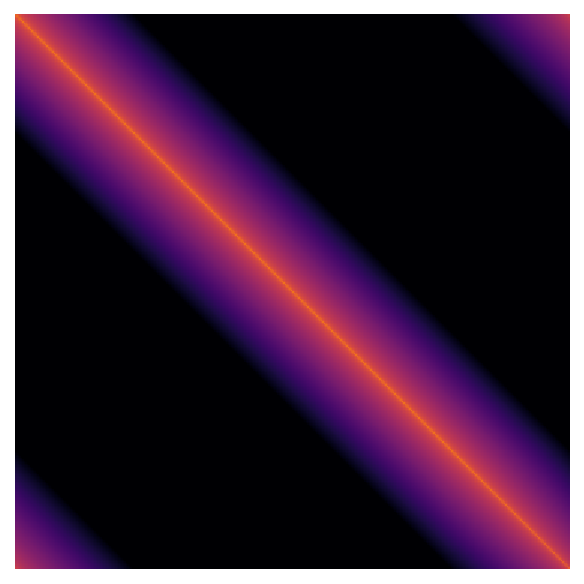
\includegraphics[width=\linewidth]{figures/G_BandMF.pdf}
        \subcaption{BandMF, $p=64$}
    \end{subfigure}\hfill
    \begin{subfigure}[t]{0.23\linewidth}
        \centering
        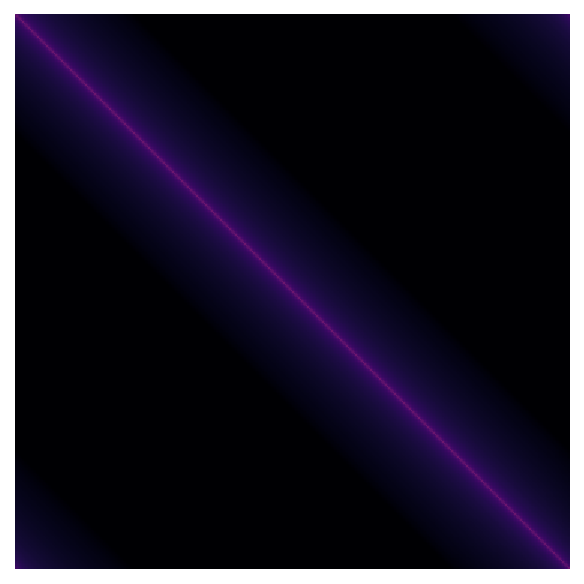
\includegraphics[width=\linewidth]{figures/G_BSR.pdf}
        \subcaption{BSR, $p=64$}
    \end{subfigure}\hfill
    \begin{subfigure}[t]{0.23\linewidth}
        \centering
        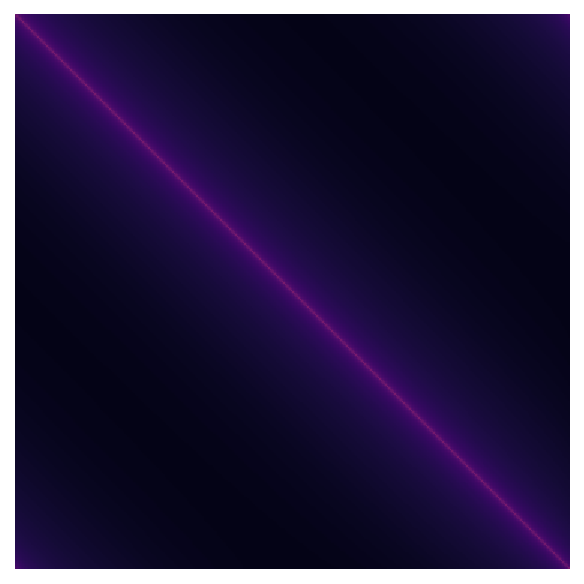
\includegraphics[width=\linewidth]{figures/G_BISR.pdf}
        \subcaption{BISR, $p=64$}
    \end{subfigure}\hfill
    \begin{subfigure}[t]{0.23\linewidth}
        \centering
        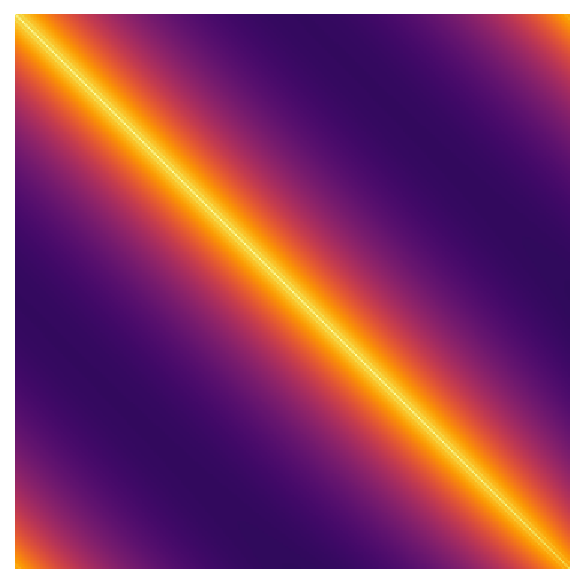
\includegraphics[width=\linewidth]{figures/G_BandInvMF.pdf}
        \subcaption{BandInvMF, $p=4$}
    \end{subfigure}

    \caption{The Gram matrix $\mathbf{G}$ for matrices of size $N=3000$ with $k=10$. For banded matrices $\mathbf{C}$, we consider Banded Matrix Factorization (BandMF) \citep{mckenna2024scaling} and Banded Square Root Factorization (BSR) \citep{kalinin2024banded} with bandwidth $p=64$. For banded inverse matrices, we consider Banded Inverse Matrix Factorization (BandInvMF) and Banded Inverse Square Root (BISR) \citep{kalinin2025back} with bandwidths $p = 4$ and $p=64$ accordingly.
  We note that although the matrix $\mathbf{C}$ is banded, the matrix $\mathbf{G}$ is not; rather, it is \emph{cyclically banded}, with the corner blocks filled by strictly positive entries. Moreover, we observe that banded inverse matrices show similar behavior: their Gram matrices have entries that decay rapidly outside the cyclic band.}
    \label{fig:gram_subplots}
\end{figure*}


Bounds on the hockey-stick divergence imply $(\varepsilon,\delta)$-differential privacy. Since it is not feasible to compute the hockey-stick divergence explicitly, we instead compute an upper bound based on the Rényi divergence. We then translate the resulting Rényi divergence bounds at order $\alpha$ into $(\varepsilon,\delta)$-differential privacy using the following theorem.


\begin{theorem}{Prop. 12 in  \citet{canonne2020discrete}.}
\label{thm:renyi_to_hockey_stick_translation}
Given two distributions $P, Q$, if $R_{\alpha}(P \,\|\, Q) \leq \rho$, then
\begin{equation}
H_{e^\epsilon}(P \,\|\, Q) \leq \frac{1}{\alpha - 1} e^{(\alpha - 1)(\rho - \epsilon)} \left(1 - \frac{1}{\alpha} \right)^{\alpha}.
\end{equation}
\end{theorem}

In the following lemma, we compute the Rényi divergence for the dominating pair from Lemma~\ref{lem:dominating_pair} 
\[
\hat{P} = \frac{1}{b}\sum_{i=1}^{b} \mathcal{N}(\mathbf{m}_i, \sigma^2 I)
\quad\text{and}\quad
\hat{Q} = \mathcal{N}(0, \sigma^2 I),
\]
in the ``remove'' direction.

\begin{restatable}{lemma}{RenyiDivergenceBound}
\label{lem:renyi-bound}
The Rényi divergence in the ``remove'' direction $R_\alpha(\hat{P}\,\|\,\hat{Q})$ is given by
\begin{equation}
\begin{aligned}
\label{eq:divergence_add}
\frac{1}{\alpha - 1}\,
\log\!\!\sum_{(r_1,\dots,r_\alpha)\in[1,b]^\alpha}
\!\!\!\!\!\exp\bigg(\!
  \sum_{\substack{j_1,j_2=1\\ j_1\ne j_2}}^\alpha
  \frac{\mathbf{G}_{r_{j_1}, r_{j_2}}}{2\sigma^2}
\!\bigg)-\frac{\alpha \log b}{1-\alpha},
\end{aligned}
\end{equation}
where $G$ is the Gram matrix with entries $\mathbf{G}_{i,j} = \langle \mathbf{m}_i, \mathbf{m}_j\rangle$.
\end{restatable}


For a general Gram matrix $\mathbf{G}$, we do not see an efficient way to evaluate this sum. The expression resembles the partition function of a probabilistic graphical model with all to all interactions, suggesting that the computation may be NP hard. However, if we impose structural restrictions on $\mathbf{C}$, for instance by requiring it to be $p$ banded, then $\mathbf{G}$ inherits additional structure and becomes \emph{cyclic banded} (see Figure~\ref{fig:gram_subplots}). In this case, the sum can be computed via dynamic programming in time $O\!\left(bp\,\alpha^{2p}\right)$. In particular, for $p=1$, which corresponds to the DP-SGD case, this yields a runtime of $O(b\alpha^2)$, improving upon the exponential $O(2^\alpha)$ complexity reported by \citet{feldman2025privacy}.

If $\mathbf{C}$ is not naturally $p$ banded, as is the case for banded inverse matrices in~\citet{kalinin2025back}, the procedure above is no longer efficient. Nevertheless, many such matrices are effectively close to banded in the sense that entries sufficiently far from the diagonal are small (see Figure~\ref{fig:gram_subplots}). This observation leads to the following bound. Let
\[
\tau \coloneqq \max_{\min(|i-j|, b - |i-j|)\ge p} \mathbf{G}_{i,j}.
\]
Then $\mathbf{G}$ admits the elementwise bound $\mathbf{G} \le \mathbf{G}^{p} + \tau \mathbf{E}$, where $\mathbf{G}^{p}$ is the $p$ cyclic banded truncation of $\mathbf{G}$ and $\mathbf{E}$ denotes the all ones matrix. Consequently, by adding an extra term $\frac{\alpha \tau}{2\sigma^2}$ to the Rényi divergence, we obtain a computable upper bound on the privacy loss.

Combining these observations, Algorithm~\ref{alg:renyi_dynamic_program} computes the Rényi divergence in the ``remove'' direction exactly when $\mathbf{C}$ is $p$ banded, and an upper bound otherwise. Formally:
%The guarantees of Algorithm~\ref{alg:renyi_dynamic_program} can be formally state as follows:


\begin{restatable}{lemma}{RenyiDynamicProgram}
\label{lem:renyi-dynamic_program}
Algorithm~\ref{alg:renyi_dynamic_program} computes the Rényi divergence based value in eq.~\ref{eq:divergence_add} exactly for a $p$-banded strategy matrix $\mathbf{C}$, and returns an upper bound otherwise.
The algorithm runs in time $O\!\left(bp \alpha^{2p} \right)$ and requires $O(\alpha^{p} + bp)$ memory.
\end{restatable}

Algorithm~\ref{alg:renyi_dynamic_program} evaluates the sum in~\eqref{eq:divergence_add} exactly when the Gram matrix $\mathbf{G}$ is $p$ cyclically banded, and returns an upper bound otherwise by truncating $\mathbf{G}$ to its $p$ cyclically banded part $\mathbf{G}^{(p)}$ and adding the correction term $\frac{\tau\alpha}{2\sigma^2}$. The indices in~\eqref{eq:divergence_add} interact cyclically; we break this cycle by conditioning on the short prefix $\mathbf{l}=(l_0,\dots,l_{p-2})$ and then compute the remaining contribution via a forward dynamic program. We glue the cycle back at the end by adding the interactions between indices $b-p+2,\dots,b-1$ and $0,\dots,p-2$. For numerical stability, all aggregations are performed using the log-sum-exp (LSE) operation. See the proof of Lemma~\ref{lem:renyi-dynamic_program} for a detailed description.


However, this is not sufficient to prove $(\varepsilon,\delta)$-DP, since the notion of neighboring datasets allows adding or removing a single element, which requires a bound in the other direction as well. We found it substantially harder to compute the divergence $\mathrm{R}_{\alpha}(\hat{Q}\,\|\,\hat{P})$ explicitly. Nevertheless, it admits a tight and easily computable upper bound, which we present in the following lemma and formalize in Algorithm~\ref{alg:renyi_dynamic_program_remove}


\begin{restatable}{lemma}{RemoveRenyiBound}
\label{lem:remove-renyi-bound}
The Rényi divergence in the ``add'' direction is bounded as
\begin{equation}
    \mathrm{R}_{\alpha}(\hat{Q}\|\hat{P})
    \le
    \frac{1}{2b\sigma^2} \sum_{j = 1}^b \mathbf{G}_{j,j}
    \;+\;
    \frac{\alpha - 1}{2b^2\sigma^2} \sum_{i = 1}^b \sum_{j = 1}^b \mathbf{G}_{i,j},
\end{equation}
where $\mathbf{G}$ is the Gram matrix with entries $\mathbf{G}_{i,j} = \langle \mathbf{m}_i, \mathbf{m}_j\rangle$.
\end{restatable}

Taking the maximum over the ``add'' and ``remove'' directions, $
\max\!\bigl(\mathrm{R}_{\alpha}(\hat{Q}\,\|\,\hat{P}),\,\mathrm{R}_{\alpha}(\hat{P}\,\|\,\hat{Q})\bigr)$, and converting it to a  hockey stick divergence via Theorem~\ref{thm:renyi_to_hockey_stick_translation} then completes the computation; see Algorithm~\ref{alg:renyi_dynamic_program_full}. To run the algorithm, we must choose the R\'enyi order $\alpha$ that yields the tightest privacy guarantee. For practical values of $\epsilon$ and $\delta$, the optimal $\alpha$ typically lies between $2$ and $40$. Theoretically, Theorem~\ref{thm:renyi_to_hockey_stick_translation} suggests that for small $\delta$, the optimal $\alpha$ grows logarithmically with $1/\delta$.



\begin{algorithm}[t!]
\caption{Rényi Accountant ``add'' direction}
\label{alg:renyi_dynamic_program_remove}
\begin{algorithmic}[1]

\REQUIRE Correlation matrix $C$, bandwidth $p$, separation $b$, parameter $\alpha \in \mathbb{N}_{+}$.

\STATE $\mathbf{m}_i \leftarrow \sum_{j=0}^{k-1} |\mathbf{C}|_{:,\, i + jb}$

\STATE $\mathbf{G}_{i,j} \leftarrow \langle \mathbf{m}_i, \mathbf{m}_j \rangle \quad \forall i,j \in \{1,\dots,b\}$

\STATE $\rho \leftarrow \frac{1}{2b\sigma^2} \sum_{j = 1}^b \mathbf{G}_{j,j}
    \;+\;
    \frac{\alpha - 1}{2b^2\sigma^2} \sum_{i = 1}^b \sum_{j = 1}^b \mathbf{G}_{i,j}$
\STATE \textbf{return} $\rho$
\end{algorithmic}
\end{algorithm}

\begin{algorithm}[t!]
\caption{Rényi Accountant Full Algorithm}
\label{alg:renyi_dynamic_program_full}
\begin{algorithmic}[1]

\REQUIRE Correlation matrix $\mathbf{C}$, bandwidth $p$, separation $b$, parameter $\alpha \in \mathbb{N}_{+}$.

\STATE $\rho_{\mathrm{remove}} \leftarrow \mathrm{ReAcc_{remove}}(\mathbf{C}, p, b, \alpha)$ \qquad \quad \, \text{\# Algorithm \ref{alg:renyi_dynamic_program}}

\STATE $\rho_{\mathrm{add}} \leftarrow \mathrm{ReAcc_{add}}(\mathbf{C}, p, b, \alpha)$ \quad \text{\# Algorithm \ref{alg:renyi_dynamic_program_remove}}

\STATE $\rho \leftarrow \max(\rho_{\mathrm{remove}}, \rho_{\mathrm{add}})$
\STATE
$\delta(\alpha,\varepsilon) \leftarrow
\exp\!\big((\rho-\varepsilon)(\alpha-1)\big)
(\alpha-1)^{-1}(1-1/\alpha)^\alpha$

\STATE \textbf{return} $\delta(\alpha,\varepsilon)$
\end{algorithmic}
\end{algorithm}



\section{Conditional Composition Accountant}
The proposed dynamic program allows for an exact evaluation of the R\'enyi divergence and thus cumulant generating function for any $\alpha_+ \in \sN_+$.\footnote{Real-valued orders $\alpha$ can be evaluated via interpolation, see Corollary 10 in~\cite{wang2019subsampled}}
These can be exactly converted to privacy profiles $\delta(\epsilon)$ via the inverse Laplace transform~\cite{zhu2022optimal}, but this is generally intractable. Conversion formulae such as~\cref{thm:renyi_to_hockey_stick_translation} sacrifice some of this tightness, and are best suited for capturing the large deviation behavior of privacy loss $L_{P,Q}$~\cite{alghamdi2023saddle}, i.e., ``large $\epsilon$''.
We therefore derive a complementary method that---as our experiments demonstrate---yields tighter bounds under strict privacy budgets, i.e., ``small $\epsilon$''.

What prevents us from using recent privacy accountants that avoid the looseness of R\'enyi conversion formulae  (e.g., convolution of privacy loss distributions~\cite{sommer2019privacyloss,koskela2020computing})
is that they assume the dominating pair to factorize into (usually univariate) per-step dominating pairs 
$P = \bigtimes_{n=1}^N P^{(n)}$ and $Q = \bigtimes_{n=1}^N Q^{(n)}$.
Matrix mechanisms and random allocation introduce shared randomness 
due to noise correlation and the fixed number of participations.
Our dominating pair from~\cref{lem:dominating_pair} thus violates this independence assumption.

Conditional composition\footnote{It is also referred to as posterior sampling in~\cite{feldman2025privacy}, following earlier work in~\cite{erlingsson2020encode}.} is a general tool for overcoming this problem of non-independence by taking an arbitrary dominating pair and upper-bounding its privacy profile with a factorizing dominating pair.
For our purposes, we use the following formulation of conditional composition (for its relation to the general Theorem, see~\cref{appendix:proofs_conditional_composition}).
\begin{restatable}{lemma}{conditionalcomposition}[Special case of Theorem 3.1 in~\cite{choquette2023privacy}]
\label{lemma:conditional_composition}
    Let $P, Q$ be distributions on $\sR^{N}$.
    For every step $n \in {N}$, choose a fixed pair of distributions $P^{(n)}, Q^{(n)}$.
    Let $A^{(n)} \subseteq \sR^N$ refer to all ``good'' outcomes $\tilde{y}$ such that
    the conditional distributions $P_{y_n | \tilde{y}_{1:n-1}}$
    and $Q_{y_n | \tilde{y}_{1:n-1}}$ are dominated by $P^{(n)}, Q^{(n)}$.
    Define ``bad'' outcomes $E = \bigcup\nolimits_{n=1}^N \overline{A^{(n)}}$ with probability $\delta_E = P(E)$.
    Then
    \begin{equation*}
        H_\gamma(P || Q) \leq H_\gamma \left( \bigtimes\nolimits_{n=1}^N P^{(n)}  || \bigtimes\nolimits_{n=1}^N  Q^{(N)} \right) + \delta_E.
    \end{equation*}
\end{restatable}
In plain terms: If we can bound the privacy of all steps independently of earlier outcomes---except for some low-probability cases $E$---then we can use standard privacy accounting at a small additional cost of $\delta_E = P(E)$.

While~\cref{lemma:conditional_composition} provides a valid composition rule, the challenge in applying it lies in 
(a) choosing appropriate per-step distributions $P^{(n)}, Q^{(n)}$
(b) analyzing the probability of them being a valid dominating pair for the conditional distribution at each step $n$, 
(c) defining a procedure for computing  the per-step dominating pairs $P^{(n)},Q^{(n)}$ and slack $\delta_E$.
We address these challenges in the following sections.
All proofs can be found in~\cref{appendix:proofs_conditional_composition}.

\subsection{Per-Step Dominating Pairs for Matrix Mechanisms}\label{section:per_step_dominating_pairs}
From the definition of $P, Q$ in~\cref{lem:dominating_pair} and the law of total probability, we know that for any previous outcome $\vy_{1:n-1} \in \sR^{n-1}$ the conditional density of step $n$ is 
\begin{align*}
    &
    p(y_n \mid \vy_{1:n-1}) = \sum_{i=1}^b \mathcal{N}(\evy_n \mid \emm_{i,n}, \sigma) p(z=i \mid \vy_{1:n-1})
    \\
    &
    q(y_n \mid \vy_{1:n-1}) = \mathcal{N}(\evy_n \mid 0, \sigma),
\end{align*}
with non-negative means $\evm_{i,n} \in \sR_+$ and 
$p(z=i) = \frac{1}{b}$, where $b$ is the number of batches per epoch.
Thus, a natural choice for our per-step dominating pair $P^{(n)}, Q^{(n)}$ is via 
\begin{align}
    &
    p^{(n)}(y_n) = \sum_{i=1}^b \mathcal{N}(\evy_n \mid \emm_{i,n}, \sigma) p^{(n)}(z=i) \label{eq:per_step_dominating_p}
    \\
    &
    q^{(n)}(y_n) = \mathcal{N}(\evy_n \mid 0, \sigma), \label{eq:per_step_dominating_q}
\end{align}
with some appropriate choice of categorical mixture weights $p^{(n)}(z=i)$.
Note that $P^{(n)}$ and $Q^{(n)}$ are fixed distributions, and specifically that the mixture weights $p^{(n)}(z=i)$ do not 
depend on earlier outcomes $\vy_{1:n-1}$.

For any \emph{fixed} $\vy_{1:n-1}$, we can test whether $P^{(n)}, Q^{(n)}$ dominate $P_{y_n | y_{1:n-1}}$
and $Q_{y_n | y_{1:n-1}}$ via the following monotonicity result,
which formalizes that having more weight on large mixture components results in a larger divergence:
\begin{restatable}{lemma}{mogweightmonotonicity}[Corollary 4.4 in~\cite{choquette2023privacy}]
    \label{lemma:stochastic_dominance_to_dp_dominance}
    Define distributions $P = \sum_{i=1}^b \mathcal{N}(\mu_i, \sigma) p(z=i)$
    and $Q = \mathcal{N}(0, \sigma)$
    with  $0 \leq \mu_b \leq \dots \leq \mu_b$.
    Let $P' = \sum_{i=1}^b \mathcal{N}(\mu_i, \sigma) p'(z=i)$.
    Then $(P, Q) \prec (P', Q)$ and $(Q, P) \prec (Q, P')$ whenever
    $p(z)$ is stochastically dominated by $p'(z)$, i.e.,
    $P(z \geq i) \leq P'(z \geq i)$ for all $i \in [b]$.
\end{restatable}
However, testing whether $P^{(n)}, Q^{(n)}$ is a valid dominating pair for a single $\vy_{1:n-1}$ is not sufficient.
To apply conditional composition, we need to know: \emph{How likely is it that $P^{(n)}, Q^{(n)})$ is a dominating pair}? That is,  how likely is it that $p(z  \mid \vy_{1:n-1})$
is stochastically dominated by $p^{(n)}(z)$ for $\vy \sim P$ or $\vy \sim Q$?\footnote{Stochastic dominance between mixture weights is not to be confused with dominance in the ``dominating pairs`` sense.}
To answer this question for the categorical distribution induced by matrix mechanisms and random allocation,
we propose to use reverse hazard functions,
i.e., the probability of the $b-i+1$-largest component
conditioned on the exclusion of even larger components.
\begin{restatable}{lemma}{reversehazarddominance}\label{lemma:reverse_hazard_to_stochastic_dominance}
    Given $p, p' : [b] \rightarrow [0,1] $, 
    define the corresponding reverse hazard functions at $i$ as  $\lambda_i = P(z = i \mid z \leq i)$ and $\lambda'_i = P'(z = i \mid z \leq i)$.
    If $\lambda_i \leq \lambda_i'$ for all $i \in [b]$, then  $p(z)$ is stochastically dominated by $p'$.
\end{restatable}
By parameterizing our per-step weights $p^{(n)}(z)$ via their reverse hazard function, we reduce the test for dominance by $P^{(n)}, Q^{(n)}$
to a pointwise comparison with the conditional reverse hazard function $P(z =i \mid z \leq i, \vy_{1:n-1})$:
\begin{restatable}{corollary}{reversehazardtodominance}\label{corollary:reverse_hazard_to_dominance}
    Assume w.l.o.g. that
    $0 \leq \emm_{1,n} \leq \dots \leq \emm_{b,n}$.
    Define arbitrary upper bounds
    $\smash{\overline{\lambda}_1, \dots \overline{\lambda}_b \in [0,1]}$ on the reverse hazard function.
    Let
    $p^{(n)}(z = i) = \overline{\lambda_i} \prod_{j=i+1}^b (1 - \overline{\lambda_i})$ and define per-step dominating pair
    $P^{(n)}, Q^{(n)}$ as in~\cref{eq:per_step_dominating_p,eq:per_step_dominating_q}.
    Whenever
    $\smash{P(z =i \mid z \leq i, \vy_{1:n-1}) \leq \overline{\lambda}_i}$ for all $\smash{i \in [b]}$, then
    $(P_{y_n | y_{1:n-1}}, Q_{y_n | y_{1:n-1}}) \prec (P^{(n)}, Q^{(n)})$
    and
    $(Q_{y_n | y_{1:n-1}}, P_{y_n | y_{1:n-1}}) \prec (Q^{(n)}, P^{(n)})$.
\end{restatable}
By applying Bayes' law, we see that this pointwise comparison between reverse hazard functions equivalent to
testing a tail bound on a specific privacy loss:
\begin{restatable}{lemma}{reversehazardloss}\label{lemma:reverse_hazard_loss}
    Let $s(x) = (1 + e^{-x})^{-1}$. 
    For any $i \in [b]$,
    the conditional reverse hazard function is 
     $P(z =i \mid z \leq i, \vy_{1:n-1}) = s(- \log(i-1) - L_i(\vy_{1:n-1}))$ with
    \begin{equation*}
        L_i(\vy_{1:n-1}) =
        \log\left(
        \frac{\sum_{j=1}^{i-1} \mathcal{N}(\vy_{1:n-1} \mid \mm_{j,:n-1}, \sigma^2 \eye)  \frac{1}{i-1}}{\mathcal{N}(\vy_{1:n-1} \mid \emm_{i,n:-1}, \sigma^2 \eye)}
        \right)
    \end{equation*}
\end{restatable}
\cref{algorithm:conditional_composition} combines the last two results to find a high-probability dominating pair $P^{(n)},Q^{(n)}$ for any step $n \in [N]$: 
For each mixture component $i \in [b]$, it first computes a lower tail bound  $\tau_i$ (which we will instantiate in~\cref{section:variational_pld_bound})
on the privacy loss $L_i$ from~\cref{lemma:reverse_hazard_loss}. It then maps it to the corresponding reverse hazard bound $\overline{\lambda_i}$ via the sigmoid function.
The sorting operation enforces the monotonicity assumption from~\cref{corollary:reverse_hazard_to_dominance}.
Correctness follows from a union bound over mixture components $i \in [b]$.
\begin{restatable}{theorem}{condcompbothcorrect}
    For the ``remove'' relation, the distributions returned by~\cref{algorithm:conditional_composition} dominate $P_{\evy_n \mid \tilde{\vy}_{1:n-1}}$ and $Q_{\evy_n \mid \tilde{\vy}_{1:n-1}}$
    with probability $1 - \beta$ under $P$.
    For the ``add'' relation, the returned distributions dominate $Q_{\evy_n \mid \tilde{\vy}_{1:n-1}}$ and $P_{\evy_n \mid \tilde{\vy}_{1:n-1}}$
    with probability $1 - \beta$ under $Q$.
\end{restatable}


\begin{algorithm}[h]
\caption{Conditional Composition Dominating Pairs}
\label{algorithm:conditional_composition}
\begin{algorithmic}
\REQUIRE Mixture means $\mm \in \sR_+^{b \times N}$, iteration $n$, batches per epoch $b$, significance $\beta$, relation $r$
    \STATE $\pi \gets \mathrm{argsort\_asc}(\mm_{:, n})$
    \STATE $\mmu_{1}, \dots, \mmu_{b} \gets \mm_{\pi(1), :n-1}, \dots, \mm_{\pi(b), :n-1}$
    \FOR{$i = b$ to $1$}
        \IF{$i = 1$}
            \STATE $\overline{\lambda}_i \gets 1$
        \ELSE
        \STATE $\tilde{P} \gets \sum_{j=1}^{i-1} \mathcal{N}(\mmu_j, \sigma^2 \eye) \cdot \frac{1}{i-1}$
        \STATE $\tilde{Q} \gets \mathcal{N}(\mmu_i, \sigma^2 \eye)$
        \IF{r = \texttt{REMOVE}}
            \STATE $\tilde{R} \gets \sum_{k=i}^{b} \mathcal{N}(\mmu_k, \sigma^2 \eye_{n-1}) \cdot \frac{1}{b}$
        \ELSE
            \STATE $\tilde{R} \gets \mathcal{N}(\vzero, \sigma^2 \eye_{n-1})$
        \ENDIF
        \STATE $L_{\tilde{P},\tilde{Q},\tilde{R}} \gets \log\left(\frac{\dd \tilde{P}}{\dd \tilde{Q}} (\vx)\right)$ with $\vx \sim \tilde{R}$
        \STATE{$\beta_i \gets \beta \mathbin{/} (b-1)$} \# Per-bound significance
        \STATE $\tau_i \gets \texttt{whp\_lower}(\mathrm{Law}(L_{\tilde{P},\tilde{Q},\tilde{R}}), \beta_i)$
        \STATE $\overline{\lambda}_i \gets \texttt{sigmoid}(- \log(i-1) - \tau_i)$  \ \# \cref{lemma:reverse_hazard_loss}
        \ENDIF
        \STATE $p_i \gets \lambda_i \cdot \prod_{j=i+1}^b (1 - \lambda_j)$ \ \# Equal to $\lambda_b$ when $i=b$
    \ENDFOR
    \IF{r = \texttt{REMOVE}}
        \STATE \textbf{return} $(\sum_{j=1}^b \mathcal{N}(\mu_j, \sigma) \cdot p_j), \mathcal{N}(0, \sigma)$
    \ELSE
        \STATE \textbf{return} $\mathcal{N}(0, \sigma), (\sum_{j=1}^b \mathcal{N}(\mu_j, \sigma) \cdot p_j)$
    \ENDIF
\end{algorithmic}
\end{algorithm}

\textbf{Use for conditional composition.}
\cref{algorithm:conditional_composition} returns a dominating pair for a single step $n$. However, \cref{lemma:conditional_composition} requires $N$ such dominating pairs to hold simultaneously with probability $1 - \delta_E$. While one could use a union bound, we found a non-uniform allocation of probability across steps to be preferable (see details in~\cref{appendix:significance_allocation}).

\textbf{Complexity.} 
When tracking $\smash{\prod_{j=i+1}^b(1-\lambda_i)}$ across components $\smash{i \in [b]}$, the 
complexity of using~\cref{algorithm:conditional_composition} for conditional composition is $\smash{\mathcal{O}(N b (\log(b) + \omega) + \kappa(N))}$,
where $\omega$ is the cost of a single tail bound,
and $\kappa(N)$ the cost of $N$-fold composition with any accountant.
Note that the cost is independent of privacy parameters $\epsilon$ and $\delta$.

\begin{figure*}[t!]
    \centering
    \begin{subfigure}[t]{0.3\linewidth}
        \centering
        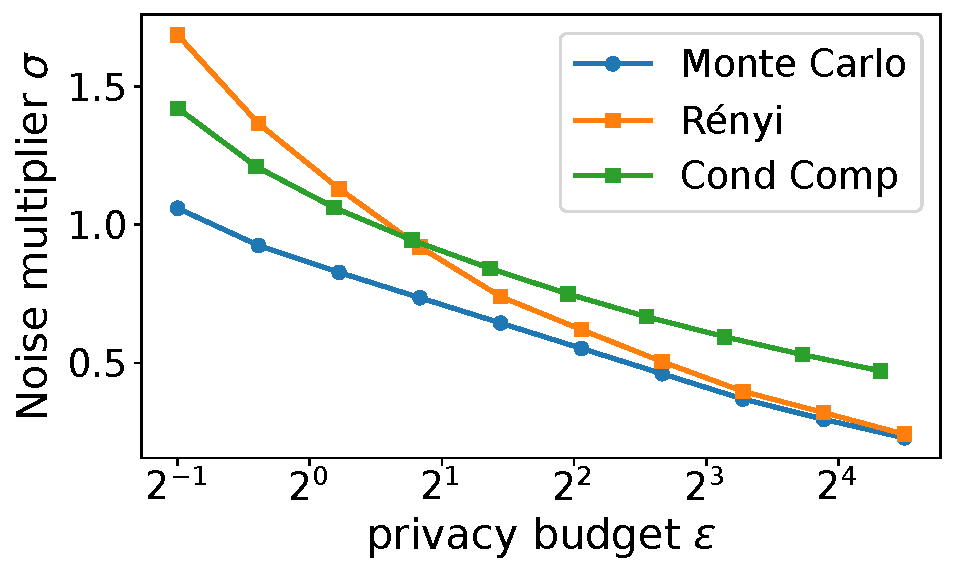
\includegraphics[width=\linewidth]{figures/sigmas_vs_epsilon_b_100_k_1_p_1_dp_sgd.pdf}
        \subcaption{DP-SGD, $N=100,\ k=1$}
         \label{fig:rdp_mcmc_dpsgd_n_100_k_1}
    \end{subfigure}\hfill
    \begin{subfigure}[t]{0.3\linewidth}
        \centering
        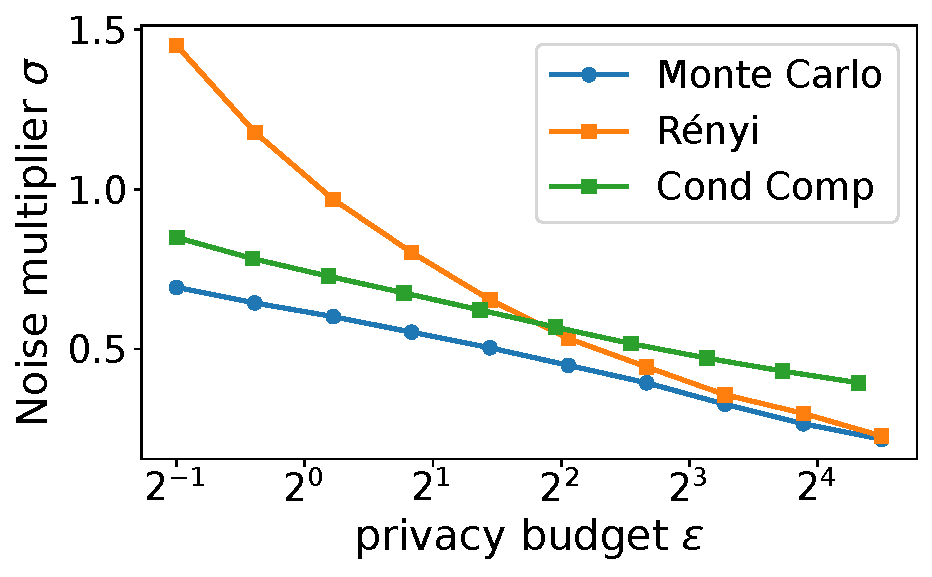
\includegraphics[width=\linewidth]{figures/sigmas_vs_epsilon_b_1000_k_1_p_1_dp_sgd.pdf}
        \subcaption{DP-SGD, $N=1000,\ k=1$}
        \label{fig:rdp_mcmc_dpsgd_n_1000_k_1}
    \end{subfigure}\hfill
    \begin{subfigure}[t]{0.3\linewidth}
        \centering
        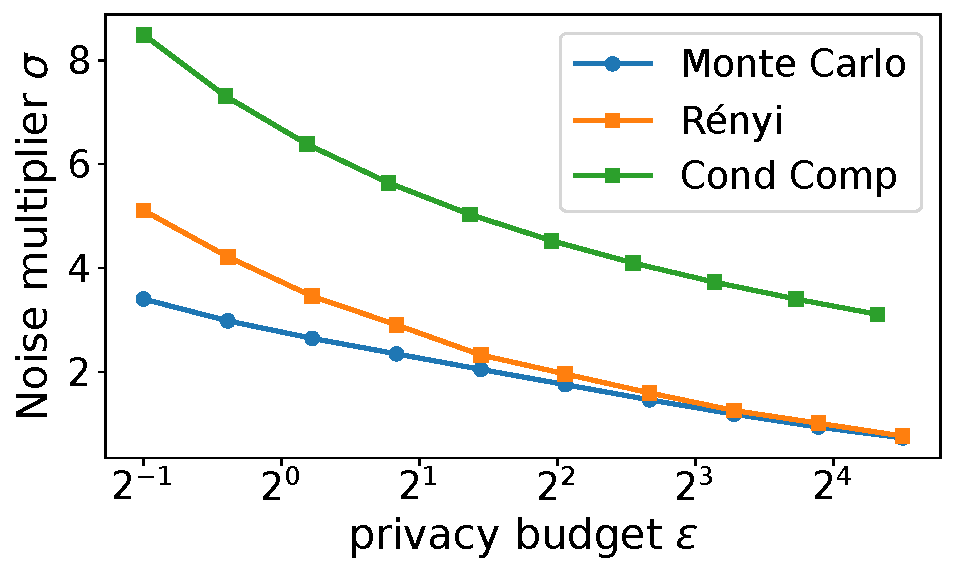
\includegraphics[width=\linewidth]{figures/sigmas_vs_epsilon_b_100_k_10_p_1_dp_sgd.pdf}
        \subcaption{DP-SGD, $N=1000,\ k=10$}
        \label{fig:rdp_mcmc_dpsgd_n_1000_k_10}
    \end{subfigure}

    
    \begin{subfigure}[t]{0.3\linewidth}
        \centering
        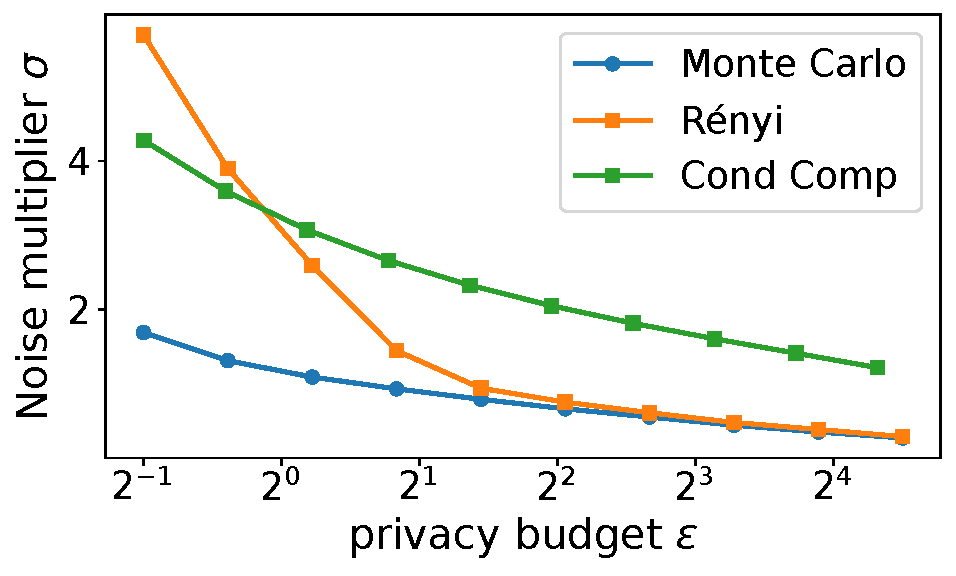
\includegraphics[width=\linewidth]{figures/sigmas_vs_epsilon_b_100_k_1_p_4_dp_bsr.pdf}
        \subcaption{BSR, $N=100,\ k=1,\ p=4$}
        \label{fig:rdp_mcmc_bsr_n_100_k_1_p_4}
    \end{subfigure}\hfill
    \begin{subfigure}[t]{0.3\linewidth}
        \centering
        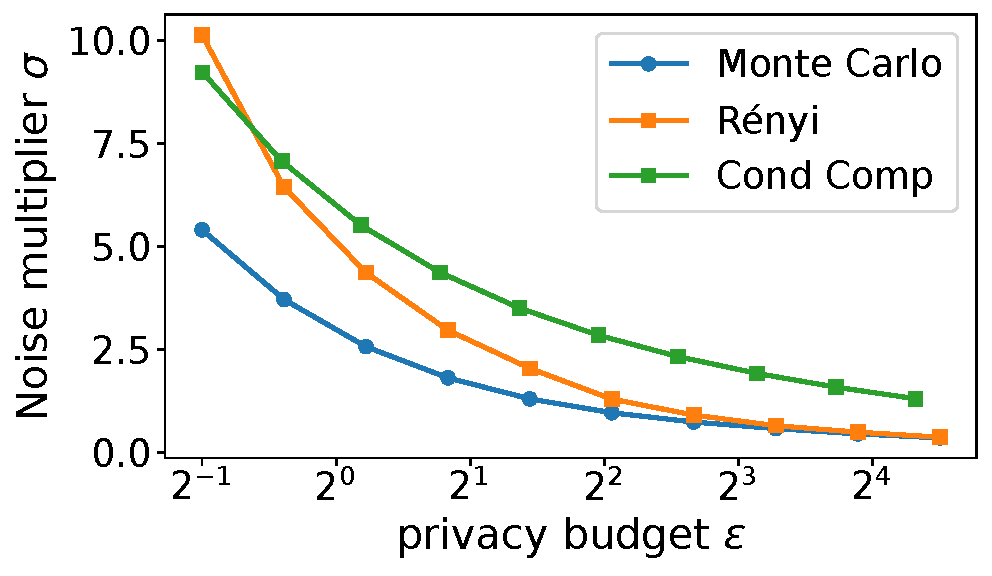
\includegraphics[width=\linewidth]{figures/sigmas_vs_epsilon_b_100_k_1_p_64_dp_bsr.pdf}
        \subcaption{BSR, $N=100,\ k=1,\ p=64$}
        \label{fig:rdp_mcmc_bsr_n_100_k_1_p_64}
    \end{subfigure}\hfill
    \begin{subfigure}[t]{0.3\linewidth}
        \centering
        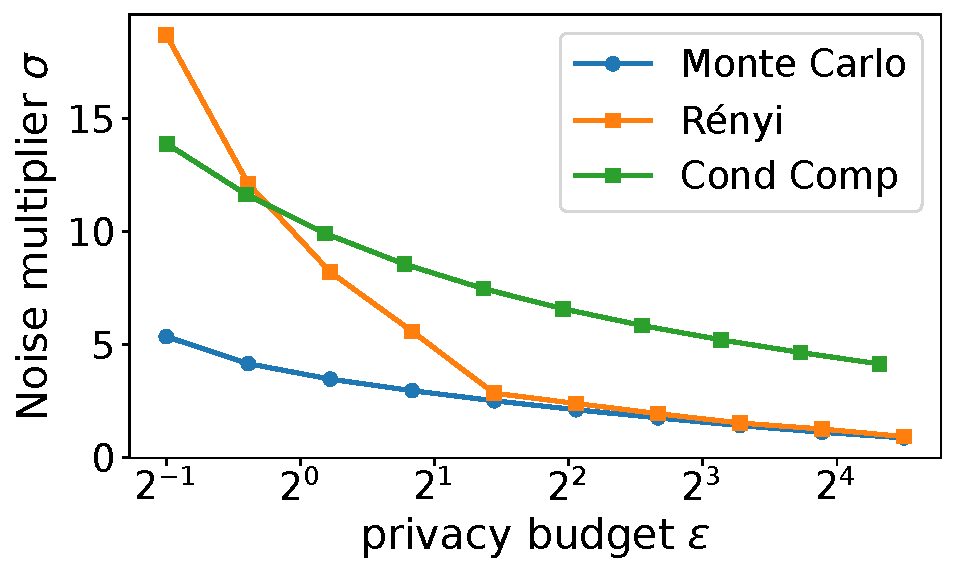
\includegraphics[width=\linewidth]{figures/sigmas_vs_epsilon_b_100_k_10_p_4_dp_bsr.pdf}
        \subcaption{BSR, $N=1000,\ k=10,\ p=4$}
        \label{fig:rdp_mcmc_bsr_n_1000_k_10_p_4}
    \end{subfigure}

    \caption{Comparison of the Rényi based and conditional composition based accountants with the Monte Carlo (MC) accountant for DP-SGD and Banded Square Root (BSR) at $\delta=10^{-5}$, with calibrated noise multipliers $\sigma$ shown as a function of the privacy budget $\varepsilon$. Each plot corresponds to a different choice of the number of iterations $n$, bandwidth $p$ and the number of epochs $k$.}
    \label{fig:rdp_mcmc_dpsgd}
    \vspace{-0.3cm}
\end{figure*}

\subsection{Variational Privacy Loss Bounds}\label{section:variational_pld_bound}
Through~\cref{algorithm:conditional_composition},
we reduce our problem of finding per-step dominating pairs to that of finding high-probability tail bounds
on a ternary form of privacy loss random variable $\smash{L_{\tilde{P},\tilde{Q},\tilde{R}} = \log( \dd \tilde{P} \mathbin{/} \dd \tilde{Q})(\vx)}$ with $\vx \sim \tilde{R}$. Specifically, $\tilde{P}$ is a uniform Gaussian mixture with means $\vmu_{1}, \dots, \vmu_{i-1}$ and $\tilde{Q}$ is a Gaussian with mean $\vmu_i$.
In the following, we present our analytical solution to this problem.
For the sake of exposition, we focus on the ``add'' case in which $\tilde{R} = \mathcal{N}(\vzero, \sigma^2 \eye)$ and discuss the  ``remove'' case in~\cref{appendix:proofs_variational}.

Characterizing the privacy loss distribution's tails is exactly what R\'enyi accounting excels at.
We could thus adapt the methods from~\cref{section:rdp_accountant} to evaluate the MGF of
$\smash{L_{\tilde{P},\tilde{Q},\tilde{R}}}$ and compute a Chernoff bound.
This is how R\'enyi accounting was originally used by~\citet{abadi2016deep} (see their Theorem 2).
However, we can also
directly exploit the approach underlying~\cref{lem:remove-renyi-bound}, bypassing the lossy Chernoff bound.
Specifically, we propose to use variational inference to find tail bounds via a tractable lower bound on the privacy loss:
\begin{restatable}{lemma}{variationalgeneric}\label{lemma:variational_generic}
    Let $\tilde{P} = \sum_{j=1}^{i-1} \mathcal{N}(\vmu_j, \sigma^2 \eye) \cdot \pi_i$
    with weights $\pi_i = \frac{1}{i-1}$ and $\tilde{Q} = \mathcal{N}(\vmu_i, \sigma^2 \eye)$.
    Let $L_i(\vx) = \log( \frac{\dd \tilde{P}}{\dd \tilde{Q}})(\vx)$ be their privacy loss at $\vx$.
    Define per-component privacy losses $
    L_{i,j}(\vx) = \log\left(\frac{ \mathcal{N}(\vx \mid \vmu_j, \sigma^2 \eye)}{\mathcal{N}(\vx \mid \vmu_i, \sigma^2 \eye)}\right)$. 
    Let $\psi$ be any categorical distribution  on $[i-1]$. Then, $L_i(\vx) \geq \underline{L_i}(\vx)$ with
    \begin{equation}\label{eq:variational_bound}
        \underline{L_i}(\vx) = \mathbb{E}_{j \sim \psi}[L_{i,j}] - \mathrm{KL}(\psi || \pi).
    \end{equation}
\end{restatable}
Because the privacy loss between two Gaussians is linear function, $\underline{L}(\vx)$ with $\vx \sim \tilde{R}$ is simply an affine transformation of a zero-mean Gaussian. We can thus show:
\begin{restatable}{theorem}{variationalboundadd}\label{theorem:variational_bound_add}
        Let $\vx \sim \tilde{R}$ with $\tilde{R} = \mathcal{N}(\vzero, \sigma^2 \eye)$.
        Then $\underline{L_i}(\vx) \sim \mathcal{N}(\nu, \xi)$ with mean and standard deviation
        \begin{align*}
            \nu &= \left(||\vmu_i||_2^2 - \mathbb{E}_{j \sim \psi}[||\vmu_j||_2^2]\right) \mathbin{/} (2 \sigma^2) - \mathrm{KL}(\psi || \pi), \\
            \xi &=   \left\lvert\left\lvert \vmu_i - \mathbb{E}_{j \sim \psi}[\vmu_j] \right\rvert\right\rvert_2 \mathbin{/} \sigma .
        \end{align*}
\end{restatable}
A tail bound with significance $\beta_i$ can thus be found analytically via the inverse CDF of $\mathcal{N}(\nu, \xi)$.
In~\cref{appendix:proofs_variational}, we analogously show for the ``remove'' case that $L_{\tilde{P},\tilde{Q},\tilde{R}}$ can be bounded
via a mixture of univariate Gaussians. There, we can find a tail bound with arbitrary precision via bisection.

\textbf{Variational family.} \cref{theorem:variational_bound_add} holds for arbitrary distributions $\psi$. 
We can thus evaluate the bound over multiple distributions from a variational family $\Psi$ and choose the best one.
We present  our choice of $\Psi$ in~\cref{appendix:choice_of_variational_family}. 


\section{Experiments}

In this section, we evaluate the R\'enyi and conditional composition (Cond Comp) based accountants against the sampling based Monte Carlo accountant \citep{choquette2024near}.
We emphasize that privacy guarantees derived via a Monte Carlo accountant are qualitatively different from the $(\epsilon,\delta)$-DP guarantees of our proposed accountants: they hold only with high probability, or require the mechanism to abstain (see~\cref{section:background_matrix_mechanisms}). We perform privacy accounting across different modern matrix mechanisms, including  
DP-SGD ($\mC = \eye$) and BSR \citep{kalinin2024banded} in~\cref{fig:rdp_mcmc_dpsgd},
as well as BISR, BandInvMF \citep{kalinin2025back}, BLT \citep{dvijotham2024efficient} and BandMF \citep{mckenna2024scaling}  in~\cref{fig:rdp_mcmc_bisr} of~\cref{appendix:extra_experiments}. 
While DP-SGD, BSR, and BISR are defined analytically,
BandMF, BandInvMF, and BLT define the entries of $\mC$ through an optimization problem (see details in~\cref{appendix:experimental_setup}).
For consistency with the experiments in~\cite{choquette2024near}, we set $\delta=10^{-5}$
and plot the required noise multiplier $\sigma$ for different $\epsilon > 0$.
This matches the practical use of DP machine learning in which we 
first define a desired level $(\epsilon,\delta)$ of privacy and then calibrate the mechanism to attain it.

Across all experiments, our R\'enyi accountant closely matches the Monte Carlo reference in the low-privacy regime (roughly $\epsilon \ge 2$--$4$), consistent with its strength in capturing large deviations. In the high-privacy regime ($\epsilon \le 1$), our conditional composition accountant yields tighter bounds and enables smaller calibrated noise multipliers, especially under stronger subsampling (larger $b$, smaller batch size). In multi-epoch settings, the same qualitative pattern holds for non-trivial matrix mechanisms (BSR/BISR), whereas for multi-epoch DP-SGD the conditional composition bound can degrade and provides little benefit over R\'enyi accounting. Finally, varying the correlation bandwidth (e.g., $p=4$ vs.\ $p=64$) does not change these conclusions: the observed low- vs.\ high-privacy behavior is robust to the strength of noise correlation.


\section{Conclusion}
The only available accountant for matrix mechanisms under balls-in-bins sampling relies on  Monte Carlo sampling \citep{choquette2024near}, which yields privacy guarantees that hold only with high probability or require random abstention. In this work, we provide a way to perform the accounting deterministically, that is, without relying on Monte Carlo sampling. Our Rényi  accountant computes the guarantees efficiently via dynamic programming, improving the time complexity for DP-SGD under random allocation \citep{feldman2025privacy} from exponential to polynomial, and generalizing the analysis to subsampled matrix mechanisms. The resulting accountant offers tight privacy guarantees in the low privacy regime.
Our conditional composition accountant upper-bounds the privacy profile via
a sequence of independent Gaussian mixture mechanisms, which lets us apply tight numerical privacy accountants and offers better guarantees in the high privacy regime.

\textbf{Limitations and future work.}
There are, however, limitations to the Rényi accountant, as the time complexity in the bandwidth is exponential, leading to a trade-off between runtime and tightness of the resulting bound. With a more efficient implementation and by allowing longer computation times, the accountant could be improved; however, the exponential dependence on bandwidth seems unavoidable.
An inherent limitation of conditional composition is that it uses a coarse partition of the co-domain into ``good'' and ``bad'' outcomes, which may result in overly pessimistic dominating pairs in the ``good case''. Future work should explore a more fine-grained partition. 
A limitation of our instantiation via variational privacy loss bounds is that
we (a) currently use a small, heuristically chosen variational family
and that (b) the underlying linear approximation is inherently conservative.
Future work should (a) consider optimization-based variational inference or
(b) directly use a tighter privacy accountant to improve the tail bounds
on the ternary privacy loss underlying the posterior.

\section*{Acknowledgments}
We thank Arun Ganesh for insightful discussions and for sharing the code for the Monte Carlo accountant.
Nikita Kalinin’s research was funded in part by the Austrian Science Fund (FWF) [10.55776/COE12].


\section*{Impact Statement}
This work advances privacy-preserving machine learning by reducing the risk that models reveal sensitive training data, while increasing the utility of the model, enabling safer and more trustworthy deployment in privacy-critical domains.

% I copied acknowledgements to a different file. I'll paste them back here again :) Just want to avoid stupid mistakes on my end leading to a desk-reject


\bibliography{references}
\bibliographystyle{icml2026}

%%%%%%%%%%%%%%%%%%%%%%%%%%%%%%%%%%%%%%%%%%%%%%%%%%%%%%%%%%%%%%%%%%%%%%%%%%%%%%%
%%%%%%%%%%%%%%%%%%%%%%%%%%%%%%%%%%%%%%%%%%%%%%%%%%%%%%%%%%%%%%%%%%%%%%%%%%%%%%%
% APPENDIX
%%%%%%%%%%%%%%%%%%%%%%%%%%%%%%%%%%%%%%%%%%%%%%%%%%%%%%%%%%%%%%%%%%%%%%%%%%%%%%%
%%%%%%%%%%%%%%%%%%%%%%%%%%%%%%%%%%%%%%%%%%%%%%%%%%%%%%%%%%%%%%%%%%%%%%%%%%%%%%%
\newpage
\appendix
\onecolumn

\section{Additional Numerical Results}\label{appendix:extra_experiments}
\begin{figure}[h!]
    \centering

    \begin{subfigure}[t]{0.3\linewidth}
        \centering
        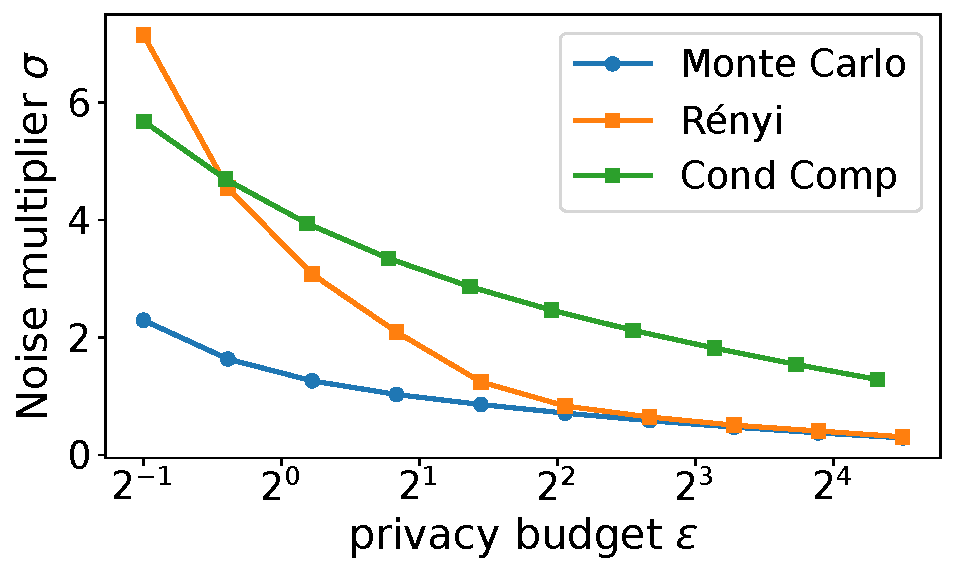
\includegraphics[width=\linewidth]{figures/sigmas_vs_epsilon_b_100_k_1_p_4_dp_bisr.pdf}
        \subcaption{BISR, $N=100,\ k=1,\ p=4$}
        \label{fig:rdp_mcmc_bisr_k_1_p_4}
    \end{subfigure}\hfill
    \begin{subfigure}[t]{0.3\linewidth}
        \centering
        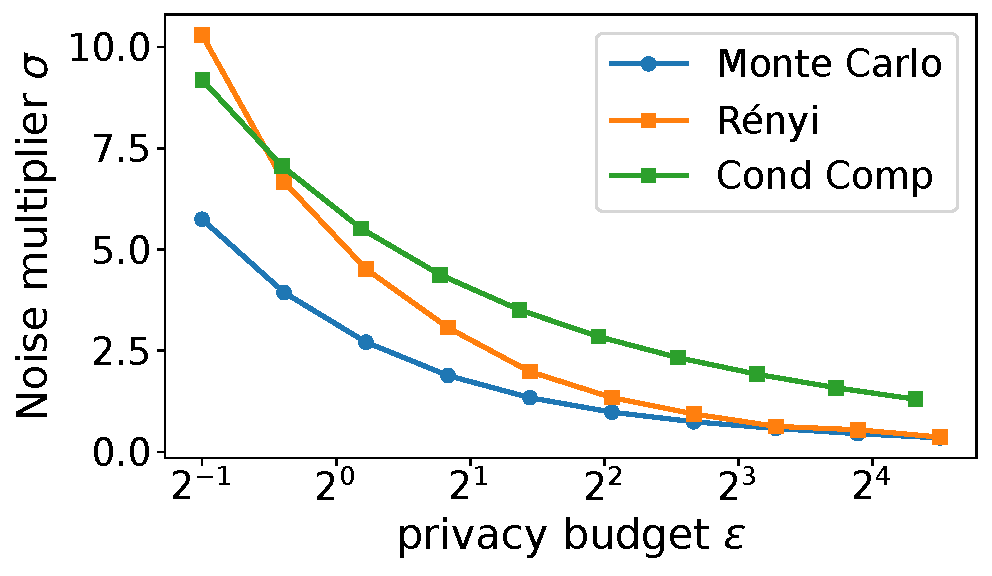
\includegraphics[width=\linewidth]{figures/sigmas_vs_epsilon_b_100_k_1_p_64_dp_bisr.pdf}
        \subcaption{BISR, $N=100,\ k=1,\ p=64$}
        \label{fig:rdp_mcmc_bisr_k_1_p_64}
    \end{subfigure}\hfill
    \begin{subfigure}[t]{0.3\linewidth}
        \centering
        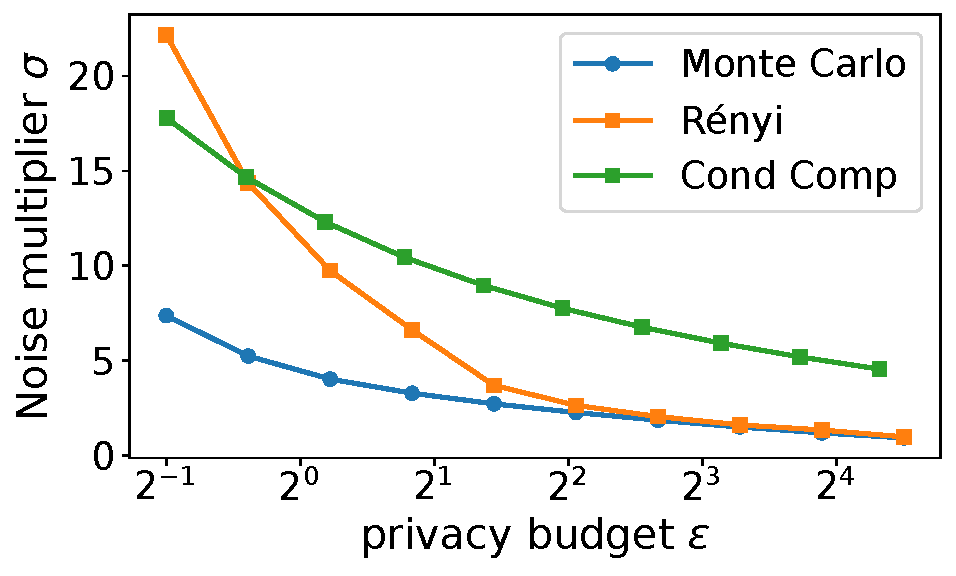
\includegraphics[width=\linewidth]{figures/sigmas_vs_epsilon_b_100_k_10_p_4_dp_bisr.pdf}
        \subcaption{BISR, $N=1000,\ k=10,\ p=4$}
        \label{fig:rdp_mcmc_bisr_k_10_p_4}
    \end{subfigure}
    
    \begin{subfigure}[t]{0.3\linewidth}
        \centering
        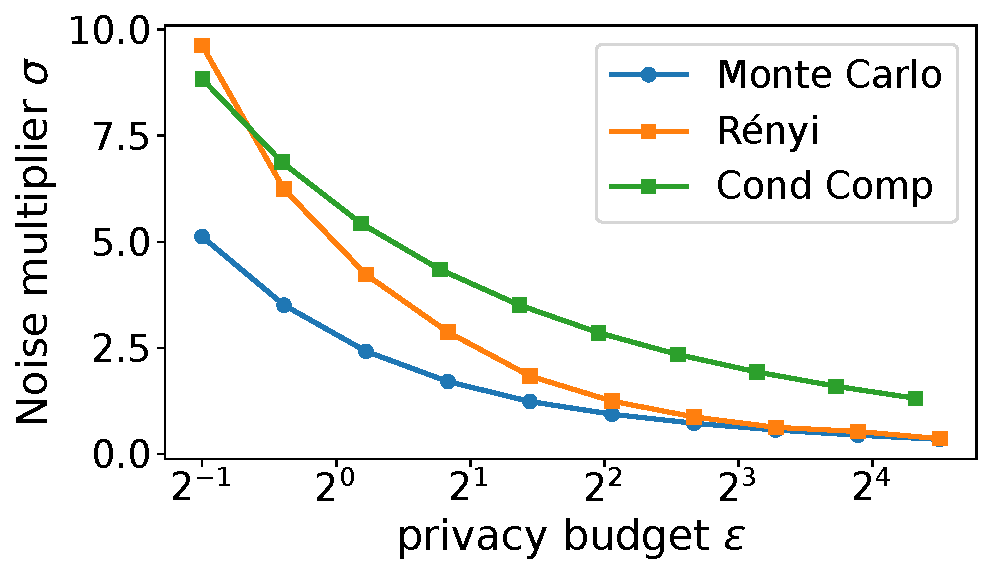
\includegraphics[width=\linewidth]{figures/sigmas_vs_epsilon_b_100_k_1_dp_blt.pdf}
        \subcaption{BLT, $N=100,\ k=1$}
    \end{subfigure}\hfill
    \begin{subfigure}[t]{0.3\linewidth}
        \centering
        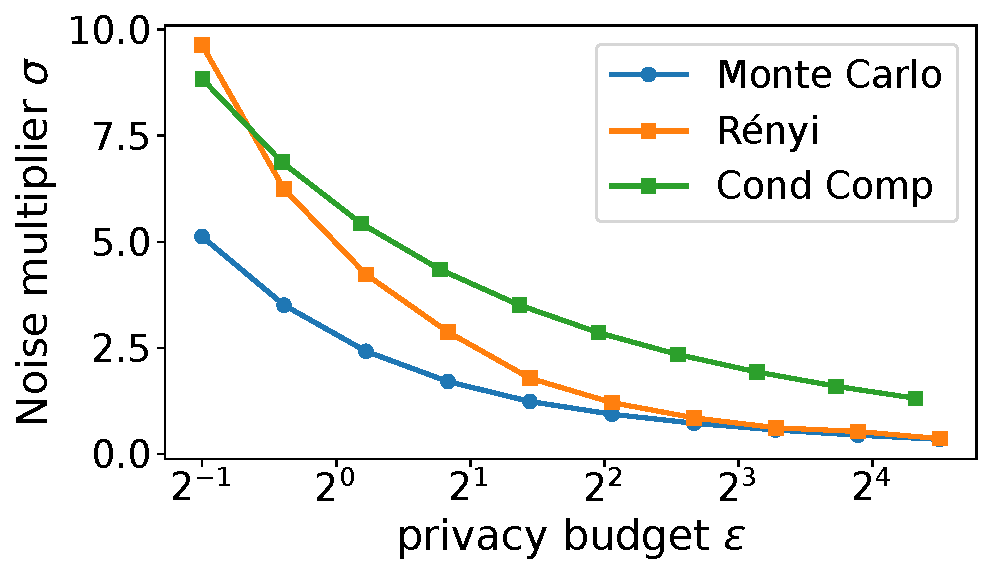
\includegraphics[width=\linewidth]{figures/sigmas_vs_epsilon_b_100_k_1_p_64_dp_bandmf.pdf}
        \subcaption{BandMF, $N=100,\ k=1,\ p=64$}
    \end{subfigure}\hfill
    \begin{subfigure}[t]{0.3\linewidth}
        \centering
        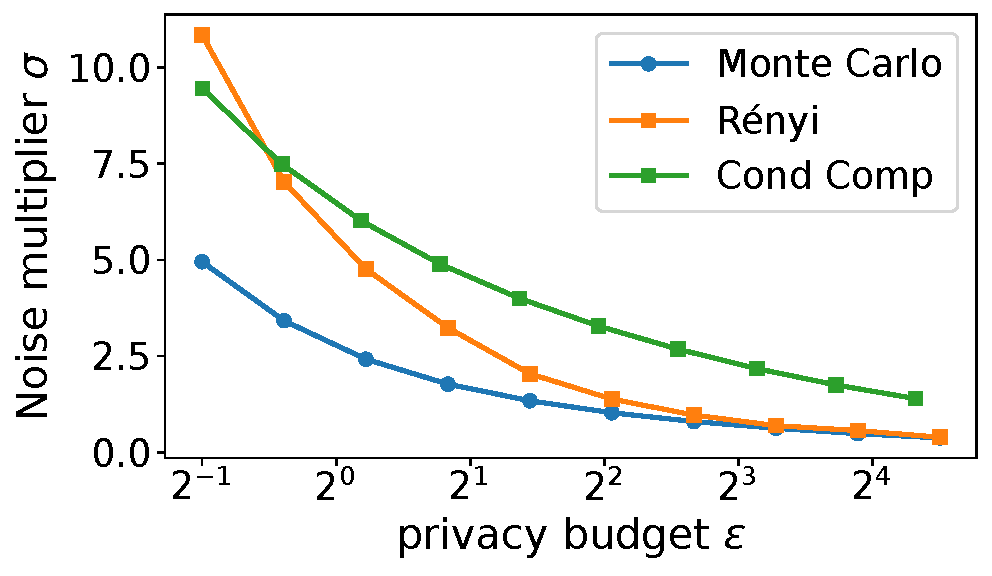
\includegraphics[width=\linewidth]{figures/sigmas_vs_epsilon_b_100_k_1_p_4_dp_bandinvmf.pdf}
        \subcaption{BandInvMF, $N=100,\ k=1,\ p=4$}
    \end{subfigure}

    \caption{Comparison of the RDP based and conditional composition based accountants with the MC accountant for BISR, BandInvMF, BLT and BandMF at $\delta=10^{-5}$, with calibrated noise multipliers $\sigma$ shown as a function of the privacy budget $\varepsilon$. Each plot corresponds to a different choice of the number of iterations $n$, the number of epochs $k$, and parameter $p$.}
    \label{fig:rdp_mcmc_bisr}
\end{figure}

\section{Experimental Details}\label{appendix:experimental_setup}
For BandMF, BLT, and BandInvMF, we use the Google \texttt{jax-privacy} implementation \citep{jaxprivacy2022github} to optimize the matrices.


\subsection{R\'enyi Accountant}
In our experiments, we have numerical trade-offs arising in privacy accounting. The R\'enyi accountant takes the bandwidth as an input. If the matrix $\mC$ is $p$-banded for a small $p$, we can compute the divergence exactly. Otherwise, when the bandwidth is large or $\mC$ is not banded, we must use an \emph{effective} bandwidth: we pass a smaller $p$ and upper bound the contributions outside the $p$-cyclic band (see Algorithm~\ref{alg:renyi_dynamic_program}). This creates a trade-off between computational cost and the tightness of the bound.

This situation occurs, for example, for banded-inverse factorizations such as BISR and BandInvMF \citep{kalinin2025back}, where $\mC^{-1}$ is banded but $\mC$ is not, and for Buffered Linear Toeplitz (BLT) \citep{dvijotham2024efficient}, which is essentially dense in both $\mC$ and $\mC^{-1}$. Moreover, smaller privacy budgets $\varepsilon$ generally require larger R\'enyi orders $\alpha$; in our experiments, the optimal $\alpha$ is typically between $30$ and $50$. In this regime, we must use a very small effective bandwidth ( $p \le 5$). In the low-privacy regime, $\alpha=2$ eventually becomes optimal, and we can afford much larger effective bandwidths (up to $p \le 25$).

\subsection{Conditional Composition Accountant}
In principle, given a target $\delta \in [0,1]$, we can choose an arbitrary ``bad'' event probability $\delta_E < \delta$
or even optimize over many different choices of $\delta_E < \delta$.
For simplicity, we follow~\cite{choquette2023privacy} and simply set $\delta_E = \delta_E \mathbin{/} 2$.

After determining per-step dominating pairs $(P^{(1)}, Q^{(1)}), \dots, (P^{(N)}, Q^{(N)})$ via~\cref{algorithm:conditional_composition}, we compute their $N$-fold composition using the Google \texttt{dp\_accounting} library~\cite{dpaccountinglibrary}  specifically its PLD accountant applied to the $\texttt{MixtureGaussianPrivacyLoss}$.
We quantize the privacy loss distribution using the ``connect the dots'' algorithm from~\cite{doroshenko2022connect},
while adjusting the value discretization interval such that each quantized privacy loss pmf has a support of size $\leq 1000$
and at least one has a support of size exactly $1000$.
We otherwise use standard parameters, in particular a log-mass truncation bound of $-50$ for the privacy loss mechanism and a 
a tail mass truncation of $\SI{1e-15}{}$ for the quantized privacy loss pmfs. 

\clearpage

\section{Proofs for Section 3}
\RenyiDivergenceBound*
\begin{proof}

By Lemma~\ref{lem:dominating_pair} $(\hat{P},\hat{Q})$ is a dominating pair for the ``add'' adjacency, where the density of $\hat{P}$ is given by
\[
p(\mathbf{x}) = \frac{1}{b}\sum_{j=1}^{b} \phi(\mathbf{x}; \mathbf{m}_j, \sigma^2 I),
\]
and the density of $\hat{Q}$ is
\[
q(\mathbf{x}) = \phi(\mathbf{x}; \mathbf{0}, \sigma^2 I),
\]
where $\phi(\mathbf{x}; \mu, \Sigma)$ denotes the density of the multivariate Gaussian distribution.

Thus, for $\alpha>1$, the Rényi divergence in the add direction is
\begin{equation}
    R_\alpha(\hat{P} || \hat{Q}) = \frac{1}{\alpha - 1} \log
    \int_{\sR^N} \frac{p(\vx)^\alpha}{q(\vx)^{\alpha-1}} \ \mathrm{d} \vx = \frac{1}{\alpha - 1} \log\mathbb{E}_{\vx \sim Q}\frac{p(\vx)^\alpha}{q(\vx)^{\alpha}}
\end{equation}
Via multinomial rule and quadratic expansion, we have
\begin{align*}
     p(\vx)^\alpha &= \left(
        \frac{1}{b}\sum_{j=1}^{b} \phi(\mathbf{x}; \mathbf{m}_j, \sigma^2 I))
    \right)^\alpha
    =
    \frac{1}{b^\alpha}
    \sum_{r_1 + \cdots + r_b = \alpha}
    \binom{\alpha}{r_1,\dots,r_b} 
    \left(\prod_{j=1}^b \phi(\mathbf{x}; \mathbf{m}_j, \sigma^2 I)^{r_j}
    \right)
    \\
    &=  \frac{1}{b^\alpha}
    \sum_{r_1 + \cdots + r_b = \alpha}
    \binom{\alpha}{r_1,\dots,r_b} \frac{1}{(2\pi\sigma^2)^{N\alpha / 2}}\exp\left(-\frac{1}{2\sigma^2}\sum\limits_{j = 1}^{b}r_j (\mathbf{x} - \vm_j )^T(\mathbf{x} - \vm_j)\right)
    \\
    &=
    \frac{1}{b^\alpha}\frac{1}{(2\pi\sigma^2)^{N\alpha / 2}}\exp\left(
        -\frac{\alpha}{2 \sigma^2} \vx^T \vx
    \right)
    \sum_{r_1 + \cdots + r_b = \alpha}
    \binom{\alpha}{r_1,\dots,r_b}
    \exp\left(
         \frac{1}{\sigma^2} \vx^T \left[\sum\limits_{j = 1}^{b} r_j \vm_j\right]
    \right)\exp \left(-\frac{1}{2\sigma^2}\sum\limits_{j = 1}^{b}r_j\vm_j^T\vm_j\right)
\end{align*}

The $q(\vx)^\alpha$ is simply given by:

\begin{equation*}
    q(\vx)^\alpha = \frac{1}{(2\pi\sigma^2)^{N\alpha / 2}}\exp\left(
        -\frac{\alpha}{2 \sigma^2} \vx^T \vx
    \right).
\end{equation*}

Then the R\'enyi divergence is computed as:
%
\begin{equation*}
     R_\alpha(\hat{P} || \hat{Q}) = \frac{1}{1 - \alpha} \log \left(\frac{1}{b^\alpha} \sum_{r_1 + \cdots + r_b = \alpha}
    \binom{\alpha}{r_1,\dots,r_b}\exp \left(-\frac{1}{2\sigma^2}\sum\limits_{j = 1}^{b}r_j\vm_j^T\vm_j\right)
    \mathbb{E}_{\vx \sim Q}\exp\left(
         \frac{1}{\sigma^2} \vx^T \left[\sum\limits_{j = 1}^{b} r_j \vm_j\right]
    \right)\right)
\end{equation*}

Using the moment generating function of a multivariate Gaussian, for $\mathbf{x}\sim \mathcal{N}(\mathbf{0}, \sigma^2 I)$ and any $\mathbf{t}\in\mathbb{R}^N$,
\[
\mathbb{E}\big[\exp(\mathbf{t}^\top \mathbf{x})\big]
=
\exp\!\left(\frac{\sigma^2}{2}\|\mathbf{t}\|_2^2\right),
\]
and taking $\mathbf{t} = \frac{1}{\sigma^2}\sum_{j=1}^{b}r_j\mathbf{m}_j$, we obtain

\begin{equation}
\label{eq:R_alpha_P_Q}
    R_\alpha(\hat{P} || \hat{Q})
    = \frac{1}{1 - \alpha} \log \left(\frac{1}{b^\alpha} \sum_{r_1 + \cdots + r_b = \alpha}
    \binom{\alpha}{r_1,\dots,r_b}\exp \left(-\frac{1}{2\sigma^2}\sum\limits_{j = 1}^{b}r_j\vm_j^T\vm_j \right)
    \exp\left(
         \frac{1}{2\sigma^2} \left\|\sum\limits_{j = 1}^{b} r_j \vm_j\right\|^2_2
    \right)\right).
\end{equation}

We change the summation from partitions of $\alpha$ to all possible $b^{\alpha}$ tuples of $\alpha$ indices in $[1, b]$:
%
\begin{align*}
    R_\alpha(\hat{P} || \hat{Q})
    &= \frac{1}{1 - \alpha} \log \left(\frac{1}{b^\alpha} \sum_{(r_1, \cdots, r_b) \in [1, b]^\alpha}
    \exp \left(-\frac{1}{2\sigma^2}\sum\limits_{j = 1}^{\alpha}\vm_j^T\vm_j \right)
    \exp\left(
         \frac{1}{2\sigma^2} \left\|\sum\limits_{j = 1}^{\alpha} \vm_j\right\|^2_2
    \right)\right)\\
    &= \frac{1}{1 - \alpha} \log \left(\frac{1}{b^\alpha} \sum_{(r_1, \cdots, r_b) \in [1, b]^\alpha}
    \exp \left(\frac{1}{2\sigma^2}\sum\limits_{j_1 \ne j_2}^{\alpha}\vm_{r_{j_1}}^T\vm_{r_{j_2}} \right)\right)\\
    &=\frac{1}{1 - \alpha} \log \left(\frac{1}{b^\alpha} \sum_{(r_1, \cdots, r_b) \in [1, b]^\alpha}
    \exp \left(\frac{1}{2\sigma^2}\sum\limits_{j_1 \ne j_2}^{\alpha}\mathbf{G}_{r_{j_1}, r_{j_2}} \right)\right),
\end{align*}
where $\mathbf{G}$ denotes the Gram matrix of vectors $\vm_j$, concluding the proof.
\end{proof}

\RenyiDynamicProgram*
\begin{proof}
    
To compute the divergence efficiently using dynamic programming, we use the expression for $R_{\alpha}(\hat{P}||\hat{Q})$ from equation~\eqref{eq:R_alpha_P_Q}, substituting the Gram matrix $\mathbf{G}$:

\begin{align}
\label{eq:r_alpha_p_q_appendix}
     R_\alpha(\hat{P} || \hat{Q}) &= \log   \sum_{r_1 + \dots  + r_b = \alpha}
    \binom{\alpha}{r_1, r_2 \dots r_{b}}
    \exp\left(
        \frac{1 }{2 \sigma^2} \sum_{j=1}^{b}r_{j}(r_{j} - 1) \mathbf{G}_{j, j} + \frac{1}{\sigma^2}\sum_{j_1 < j_2}^{b} \mathbf{G}_{j_1, j_2}r_{j_1}r_{j_2}
    \right)\\
    & = \log (\alpha!) + \log   \sum_{r_1 + \dots  + r_b = \alpha}
    \frac{1}{r_1! \dots r_{b}!}
    \exp\left(
        \frac{1 }{2 \sigma^2} \sum_{j=1}^{b}r_{j}(r_{j} - 1) \mathbf{G}_{j, j} + \frac{1}{\sigma^2}\sum_{j_1 < j_2}^{b} \mathbf{G}_{j_1, j_2}r_{j_1}r_{j_2}
    \right)
\end{align}

Next, we factor out the dependence on $r_b$, using that the matrix $\mathbf{G}$ is $p$ cyclic-banded:

\begin{align}
     &\log \sum\limits_{r_b = 0}^{\alpha}\Bigg[\frac{1}{r_{b}!} \exp\left(\frac{1}{2\sigma^2}(r_{b} - 1)r_b \mathbf{G}_{b, b} + \frac{1}{\sigma^2}\sum\limits_{j = b - p + 1}^{b - 1}r_{b} r_{j}\mathbf{G}_{j, b} + \frac{1}{\sigma^2}\sum\limits_{j = 1}^{\min(p - 1, b - p)}r_{b} r_{j}\mathbf{G}_{j, b}\right) \\
     &\quad \times \sum_{r_1 + \dots  + r_{b-1} = \alpha - r_b}
    \frac{1}{r_1! \dots r_{b - 1}!}
    \exp\left(
        \frac{1}{2 \sigma^2} \sum_{j=1}^{b - 1}r_{j}(r_{j} - 1) \mathbf{G}_{j, j} + \frac{1}{\sigma^2}\sum_{j_1 < j_2}^{b -1} \mathbf{G}_{j_1, j_2}r_{j_1}r_{j_2}
    \right)\Bigg] + \log (\alpha!)
\end{align}

This suggests a dynamic programming formulation. Define

\begin{equation}
    F(k, m, \mathbf{l}, \mathbf{r}) := \log \sum\limits_{\substack{r_1 + \dots + r_{k} = m\\ r_1, \dots r_k \ge 0\\ (r_{k - p +1}, \dots, r_{k}) = \mathbf{r}\\
    (r_1, \dots, r_{p - 1}) = \mathbf{l}\\}}\frac{1}{r_1! \dots r_{k}!}
    \exp\left(
        \frac{1 }{2 \sigma^2} \sum_{j=1}^{k}r_{j}(r_{j} - 1) \mathbf{G}_{j, j} + \frac{1}{\sigma^2}\sum_{j_1 < j_2}^{k} \mathbf{G}_{j_1, j_2}r_{j_1}r_{j_2}
    \right),
\end{equation}
where $\mathbf{l}$ is the prefix of length $p-1$ (empty if we run DP-SGD with $p=1$), and $\mathbf{r}$ is the suffix of length $p-1$ starting at position $k-p+1$.



If we compute all $O(b\alpha^{2p - 1})$ values of $F$, then the divergence is: 
%
\begin{equation}
    R_\alpha(\hat{P} || \hat{Q}) = \frac{1}{\alpha - 1} \log \sum\limits_{\|\mathbf{l}\cup \mathbf{r} \|_1 \le \alpha} \exp(F(B, \alpha, \mathbf{l}, \mathbf{r}))\exp \left(\frac{1}{\sigma^2}\sum\limits_{j_1 = 1}^{p - 1}\sum\limits_{j_2 =b - p + 2}^{b} \mathbf{G}_{j_1, j_2} l_{j_1} r_{j_2} \right)  + \frac{\log (\alpha!)}{\alpha - 1} - \frac{\alpha \log b}{\alpha - 1}.
\end{equation}

The interaction for the indices $1\le j_1 < j_2 \le b$ are accounted in the dynamic function $F$, and to compute the whole sum we would have to account for the cyclic interaction between the last $p - 1$ indices and the first $p - 1$ indices. Note that we must fix the prefix $\mathbf{l}$; otherwise, when computing the cyclic interaction, we would obtain conflicting values for the first $p-1$ entries. Although this increases the computational complexity, we view it as an unavoidable cost of cyclic interaction.



To compute the dynamic values $F$, we use dynamic programming in a forward direction. We go in a cycle over all possible prefix values $\mathbf{l} = (r_1, \dots, r_{p - 1})$. Given a state $ (k, m, \mathbf{l}, \mathbf{r})$,
we update all successor states $(k + 1, m + r_{k+1}, \mathbf{l}, (r_{k - p + 3}, \dots, r_{k+1}))$ via
\begin{align}
    &F(k + 1, m + r_{k + 1}, \mathbf{l}, (r_{k - p + 3}, \dots, r_{k +1}))\\
    &\qquad\mathrel{{+}{=}} F(k, m,  \mathbf{l}, (r_{k - p + 2}, \dots r_{k})) - \log (r_{k + 1}!) + \frac{1}{2\sigma^2}(r_{k + 1} - 1)r_{k + 1} \mathbf{G}_{k + 1, k + 1} + \frac{1}{\sigma^2}\sum\limits_{j_1 = k - p + 2}^{k}r_{k + 1} r_{j_1}\mathbf{G}_{j_1, k + 1}.
\end{align}

Each of $O(b \cdot \alpha \cdot \alpha^{p - 1} \cdot \alpha^{p - 1})$ states can be computed in $O(p)$ time, with $O(\alpha)$ forward transitions, resulting in overall runtime $O(bp \alpha^{2p})$. Regarding the memory requirements, we loop over the prefix values $\mathbf{l}$ and therefore do not need to store values for previously processed prefixes. Likewise, since we increase $k$ iteratively, we do not need to retain values from earlier $k$. Instead, we store all current suffixes (there are $O(\alpha^{p-1})$ of them), each with at most $O(\alpha)$ distinct partial sums, for a total of $O(\alpha^{p})$ memory. In addition, we must store the $p$-cyclic banded matrix $\mathbf{G}$, which requires $O(bp)$ memory, resulting in an overall requirement of $O(\alpha^{p} + bp)$ memory.


Algorithm~\ref{alg:renyi_dynamic_program} computes the sum in~\eqref{eq:r_alpha_p_q_appendix} via dynamic programming under the assumption that the Gram matrix $\mathbf{G}$ is $p$ cyclically banded, and otherwise adds the nonzero term $\frac{\tau\alpha}{2\sigma^2}$ to obtain an upper bound. Concretely, given a matrix $\mathbf{C}$, it first computes the Gram matrix $\mathbf{G}$, then forms the truncated $p$ cyclically banded matrix $\mathbf{G}^{(p)}$ together with the error term $\tau$.

The indices in the sum form a cyclic interaction. To compute the sum dynamically, we first break the cycle by looping over all prefixes $\mathbf{l}=(l_0,\dots,l_{p-2})$ whose total sum is less than the target sum $\alpha$. For each fixed prefix, we precompute the log sum of exponentials corresponding to the interactions among the first $p-1$ indices. We then expand the range of indices up to $b-1$ iteratively by running a forward dynamic program over $k=p-1,\dots,b-1$. At step $k$, the set of dynamic states is stored in a dictionary, where each state is identified by (i) the current suffix $\mathbf{r}$ of the previous $p-1$ values and (ii) the current partial sum $m$ of indices up to position $k-1$. From a state $(\mathbf{r},m)$ we propose a next value $t\in\{0,\dots,\alpha-m\}$, compute the contribution corresponding to interactions involving the new index $k$, and update the suffix, the partial sum, and the accumulated log value. For numerical stability, we aggregate contributions using the log-sum-exp (LSE) operation. The resulting states are stored in a temporary dictionary $\mathrm{new\_states}$, and $\mathrm{states}$ is updated after all admissible forward values have been considered. This completes the computation of all interactions between indices $0\le i<j\le b-1$ except for the cyclic terms. Finally, we close the cycle by adding the interactions between the final suffix and the fixed prefix in a last loop. Summing the resulting log values over all valid choices of the prefix $\mathbf{l}$ completes the computation.
 

\end{proof}

\RemoveRenyiBound*
\begin{proof}
If $(\hat{P},\hat{Q})$ is a dominating pair for the ``remove'' adjacency, then Lemma~29 of \citet{zhu2022optimal} implies that $(\hat{Q},\hat{P})$ is a dominating pair for the ``add'' adjacency.
The density of $\hat{P}$ is
\[
p(\mathbf{x}) = \frac{1}{b}\sum_{j=1}^{b} \phi(\mathbf{x}; \mathbf{m}_j, \sigma^2 I),
\]
and the density of $\hat{Q}$ is
\[
q(\mathbf{x}) = \phi(\mathbf{x}; \mathbf{0}, \sigma^2 I),
\]
where $\phi(\mathbf{x}; \mu, \Sigma)$ denotes the density of the multivariate Gaussian distribution.

Thus, for $\alpha>1$, the Rényi divergence in the remove direction is
\begin{equation}
    \mathrm{R}_{\alpha}(Q\|P)
    =
    \frac{1}{\alpha - 1}\log \int_{\mathbb{R}^{b}} \frac{q(\mathbf{x})^{\alpha}}{p(\mathbf{x})^{\alpha - 1}}\,d\mathbf{x}.
\end{equation}
The mixture density $p(\mathbf{x})$ appears in the denominator, which makes the integral difficult to compute in closed form. We therefore upper bound it.

By the arithmetic mean--geometric mean inequality (equivalently, Jensen's inequality for the exponential function),
\begin{align}
    p(\mathbf{x})
    &=
    \frac{1}{b}\sum_{j=1}^{b} \phi(\mathbf{x}; \mathbf{m}_j, \sigma^2 I)
    \;\ge\;
    \left(\prod_{j=1}^{b}\phi(\mathbf{x}; \mathbf{m}_j, \sigma^2 I)\right)^{1/b}
    \\
    &=
    \frac{1}{(2\pi \sigma^2)^{N/2}}
    \exp\!\left(
    -\frac{1}{2b\sigma^2}\sum_{j = 1}^{b}(\mathbf{x}- \mathbf{m}_j)^\top(\mathbf{x}- \mathbf{m}_j)
    \right),
\end{align}
and
\begin{equation}
    q(\mathbf{x})
    =
    \phi(\mathbf{x}; \mathbf{0}, \sigma^2 I)
    =
    \frac{1}{(2\pi \sigma^2)^{N/2}}
    \exp\!\left(-\frac{1}{2\sigma^2} \mathbf{x}^\top\mathbf{x}\right).
\end{equation}

Substituting the lower bound on $p(\mathbf{x})$ into the expression for $\mathrm{R}_{\alpha}(\hat{Q}\|\hat{P})$ yields
\begin{align}
    \mathrm{R}_{\alpha}(\hat{Q}\|\hat{P})
    &\le
    \frac{1}{\alpha - 1}
    \log\int_{\mathbb{R}^N}
    q(\mathbf{x})
    \exp\!\left(
    \frac{\alpha - 1}{2b\sigma^2}
    \sum_{j = 1}^b \bigl(-2\mathbf{x}^\top \mathbf{m}_j + \mathbf{m}_j^\top \mathbf{m}_j\bigr)
    \right)\,d\mathbf{x}
    \\
    &=
    \frac{1}{2b\sigma^2}\sum_{j = 1}^{b} \mathbf{m}_j^\top \mathbf{m}_j
    +
    \frac{1}{\alpha - 1}
    \log
    \mathbb{E}_{\mathbf{x}\sim Q}
    \exp\!\left\{
    -\frac{\alpha - 1}{b\sigma^2}
    \left(\sum_{j = 1}^{b} \mathbf{m}_j \right)^\top \mathbf{x}
    \right\}.
\end{align}

Using the moment generating function of a multivariate Gaussian, for $\mathbf{x}\sim \mathcal{N}(\mathbf{0}, \sigma^2 I)$ and any $\mathbf{t}\in\mathbb{R}^N$,
\[
\mathbb{E}\big[\exp(\mathbf{t}^\top \mathbf{x})\big]
=
\exp\!\left(\frac{\sigma^2}{2}\|\mathbf{t}\|_2^2\right),
\]
and taking $\mathbf{t} = -\frac{\alpha - 1}{b\sigma^2}\sum_{j=1}^{b}\mathbf{m}_j$, we obtain
\begin{align}
    \mathrm{R}_{\alpha}(\hat{Q}\|\hat{P})
    &\le
    \frac{1}{2b\sigma^2}\sum_{j = 1}^{b} \mathbf{m}_j^\top \mathbf{m}_j
    +
    \frac{1}{\alpha - 1}
    \cdot
    \frac{\sigma^2}{2}
    \left\|
    \frac{\alpha - 1}{b\sigma^2}
    \sum_{j = 1}^{b}\mathbf{m}_j
    \right\|_2^2
    \\
    &=
    \frac{1}{2b\sigma^2}\sum_{j = 1}^{b} \mathbf{m}_j^\top \mathbf{m}_j
    +
    \frac{\alpha - 1}{2b^2\sigma^2}
    \left\|
    \sum_{j = 1}^{b}\mathbf{m}_j
    \right\|_2^2.
\end{align}

Finally, let $G$ be the Gram matrix with entries $\mathbf{G}_{i,j} = \langle \mathbf{m}_i, \mathbf{m}_j\rangle$. Then
\[
\sum_{j=1}^{b}\mathbf{m}_j^\top\mathbf{m}_j = \sum_{j=1}^{b} \mathbf{G}_{j,j},
\qquad
\left\|\sum_{j=1}^{b}\mathbf{m}_j\right\|_2^2
=
\sum_{i=1}^{b}\sum_{j=1}^{b} \mathbf{G}_{i,j},
\]
which proves the claim.
\end{proof}

\clearpage

\section{Proofs for Section 4}\label{appendix:proofs_conditional_composition}

In the following, we first confirm that the conditional composition~\cref{lemma:conditional_composition} immediately follows as a special case of the general conditional composition framework from~\cite{choquette2023privacy}. In the next sections, we then provide the omitted proofs for our instantiation of the conditional composition framework.

The general conditional composition result is:
\begin{theorem}[Theorem 3.1 in~\cite{choquette2023privacy}]\label{thm:conditioningtrick}
Let $\mathcal{M}_1: \mathcal{D} \rightarrow \mathcal{X}_1, \mathcal{M}_2: \mathcal{X}_1 \times \mathcal{D} \rightarrow \mathcal{X}_2, \mathcal{M}_3: \mathcal{X}_1 \times \mathcal{X}_2 \times \mathcal{D} \rightarrow \mathcal{X}_3, \ldots \mathcal{M}_N$ be a sequence of adaptive mechanisms, where each $\mathcal{M}_n$ takes a dataset in $\mathcal{D}$ and the output of mechanisms $\mathcal{M}_1, \ldots, \mathcal{M}_{n-1}$ as input. Let $\mathcal{M}$ be the mechanism that outputs $(x_1 = \mathcal{M}_1(D), x_2 = \mathcal{M}_2(x_1, D), \ldots, x_N = \mathcal{M}_N(x_1, \ldots, x_{N-1}, D))$. Fix any two adjacent datasets $D, D'$. 

Suppose there exists ``bad events'' $E_1 \subseteq \mathcal{X}_1, E_2 \subseteq \mathcal{X}_1 \times \mathcal{X}_2, \ldots... E_{N-1} \subseteq \mathcal{X}_1 \times \mathcal{X}_2 \times \ldots \times \mathcal{X}_{N-1}$ such that \[\Pr_{x \sim \mathcal{M}(D)}\left[\exists n: (x_1, x_2, \ldots x_n) \in E_n\right] \leq \delta\] and pairs of distributions $(P_1, Q_1), (P_2, Q_2), \ldots (P_N, Q_N)$ such that the PLD of $\mathcal{M}_1(D)$ and $\mathcal{M}_1(D')$ is dominated by the PLD of $P^{(1)}, Q^{(1)}$ and for any $n \geq 1$ and ``good'' output $(x_1, x_2, \ldots x_n) \notin E_n$, the PLD of $\mathcal{M}_{n+1}(x_1, \ldots, x_n, D)$ and $\mathcal{M}_{n+1}(x_1, \ldots, x_n, D')$ is dominated by the PLD of $P^{(n+1)}, Q^{(n+1)}$. Then for all $\epsilon$:

\[H_\epsilon(\mathcal{M}(D), \mathcal{M}(D')) \leq H_\epsilon\left(P^{(1)} \times P^{(2)} \times \ldots \times P^{(N)}, Q^{(1)} \times Q^{(2)} \times \ldots \times Q^{(N)}\right) + \delta.\]
\end{theorem}
In our case, we do not have a mechanism, but only its dominating pair $(P, Q)$ from~\cref{lem:dominating_pair}.
However, for any $D, D'$, we can define the dummy mechanism $\mathcal{M}(D) = P$ and $\mathcal{D}' = Q$ and $M_{n}(x_1,\dots,x_n, D) = P_{x_n \mid x_{1:n-1}}$ and $M_{n}(x_1,\dots,x_n, D') = Q_{x_n \mid x_{1:n-1}}$. The special case below then follows immediately.
\conditionalcomposition*


\subsection{Proofs for Section 4.1}\label{appendix:proofs_cond_comp_algorithm}

\reversehazarddominance*
\begin{proof}
    Let $F_i = P(z \leq i)$ denote the CDF of $z$. By definition, $\lambda_i = P(z=i \mid z \leq i) = P(z=i)/F_i$.
    Furthermore, $F_{i} = F_{i+1} - P(z=i+1)$.
    It thus follows that $F_{i} = F_{i+1} - P(z=i+1) = F_{i+1}(1 - \lambda_{i+1})$. Since $F_i=1$ for any $i \geq b$, recursive application of this equality yields $F_i = \prod_{j=i+1}^b (1 - \lambda_j)$.
    The condition $\lambda_j \leq \lambda'_j$ implies $(1 - \lambda_j) \geq (1 - \lambda'_j)$ for all $j$. Consequently, $F_i \geq F'_i$ for all $i$, i.e., $p(z)$ is stochastically dominated by $p'(z)$.
\end{proof}

For the next result (\cref{corollary:reverse_hazard_to_dominance}), we first recall~\cref{lemma:stochastic_dominance_to_dp_dominance}, which relates stochastic dominance between mixture weights to dominance between Gaussian mixture mechanisms in the differential privacy sense:
\mogweightmonotonicity*

\reversehazardtodominance*
\begin{proof}
    Let $p(z)$ denote the conditional mixture weights $p(z \mid \vy_{1:n-1})$ and use $\lambda_i = P(z = i \mid i \leq i, \vy_{1:n-1})$ to denote the corresponding reverse hazard function.
    By assumption, the unconditional mixture weights we construct are $p^{(n)}(z = i) = \overline{\lambda_i} \prod_{j=i+1}^b (1 - \overline{\lambda_i})$.
    From the definition of conditional probability and the recurrence relation $F_i = \prod_{j=i+1}^b (1 - \lambda_j)$ used in our previous proof, it follows that the corresponding reverse hazard function is:
    \begin{equation*}
        P^{(n)}(z = i \mid z \leq i) = \frac{p^{(n)}(z = i)}{F_i} =
            \frac{
                \overline{\lambda_i} \prod_{j=i+1}^b (1 - \overline{\lambda_i})
            }{
                \prod_{j=i+1}^b (1 - \lambda_j)
            }
            = \overline{\lambda_i}.
    \end{equation*}
    That is, $\overline{\lambda_i}$ is exactly the reverse hazard function of $p^{(n)}$.
    By assumption, $\lambda_i \leq \overline{\lambda_i}$.
    It thus follows from~\cref{lemma:reverse_hazard_to_stochastic_dominance}
    that $p(z)$ is stochastically dominated by $p^{(n)}$.
    The result is then an immediate consequence of~\cref{lemma:stochastic_dominance_to_dp_dominance}.
\end{proof}

\reversehazardloss*
\begin{proof}
    Let $p(\vy_{1:n-1} \mid z=j) = \mathcal{N}(\vy_{1:n-1} \mid \bm{m}_{j,:n-1}, \sigma^2 \eye)$ denote the likelihood of the earlier outcome $\vy_{1:n-1}$ conditioned on mixture component $j$.
    Let $p(z=j) = \frac{1}{b}$ denote the uniform prior that arises from random allocation with $b$ batches per epoch.
    Using the definition of conditional probability and Bayes' rule, the conditional reverse hazard function is:
    \begin{align*}
        &\Pr(z=i \mid z \leq i, \vy_{1:n-1})\\
        = &\frac{p(\vy_{1:n-1} \mid z=i)  p(z=i)}{\sum_{j=1}^i p(\vy_{1:n-1} \mid z=j)  p(z=j)}\\
        =& \frac{p(\vy_{1:n-1} \mid z=i)}{\sum_{j=1}^i p(\vy_{1:n-1} \mid z=j)}\\
        = & \left(1 + \frac{\sum_{j=1}^{i-1} p(\vy_{1:n-1} \mid z=j)}{p(\vy_{1:n-1} \mid z=i)}\right)^{-1}.
    \end{align*}
    Recall that $L_i(\vy_{1:n-1}) = \log \left( \frac{\frac{1}{i-1}\sum_{j=1}^{i-1} p(\vy_{1:n-1} \mid z=j)}{p(\vy_{1:n-1} \mid z=i)} \right)$.
    Multiplying and dividing the second summand by $i-1$ yields:
    \begin{equation}
        \frac{\sum_{j=1}^{i-1} p(\vy_{1:n-1} \mid z=j)}{p(\vy_{1:n-1} \mid z=i)}
        = (i-1) \exp(L_i(\vy_{1:n-1}))
        = \exp(\log(i-1) + L_i(\vy_{1:n-1})).
    \end{equation}
    Applying the definition of the sigmoid function $s(x) = (1+e^{-x})^{-1}$, we obtain:
    \begin{equation}
        \Pr(z=i \mid z \leq i, \vy_{1:n-1}) = s\left(-\big(\log(i-1) + L_i(\vy_{1:n-1})\big)\right),
    \end{equation}
    which completes the proof.
\end{proof}

While~\cref{section:per_step_dominating_pairs} in its entirety already served as a proof sketch,
we now provide a formal proof for the correctness of~\cref{algorithm:conditional_composition}:
\condcompbothcorrect*
\begin{proof}
    \cref{algorithm:conditional_composition} allocates a failure probability $\beta_i$ to each component $i$ such that $\sum_{i} \beta_i = \beta$.
    For each $i$, the subroutine \texttt{whp\_lower} returns a threshold $\tau_i$ such that $\Pr[L_i(\vy_{1:n-1}) < \tau_i] \leq \beta_i$, where the probability is over the randomness of the privacy loss random variable $L_{\tilde{P},\tilde{Q},\tilde{R}}$ generated by the algorithm's reference distribution $\tilde{R}$.
    In the ``remove'' case, $\tilde{R}$ is the joint distribution $P_{\vy_{1:n-1}}$ of the first $n-1$ outcomes of $\vy \sim P$.
    In the ``add'' case, $\tilde{R}$ is the joint distribution $Q_{\vy_{1:n-1}}$ of the first $n-1$ outcomes of $\vy \sim Q$.


    Define the failure event $\overline{A} = \bigcup_i \{ L_i(\vy_{1:n-1}) < \tau_i \}$
    with $L_i$ defined in~\cref{lemma:reverse_hazard_loss}. By a union bound, $\Pr(\overline{A}) \leq \sum \beta_i = \beta$.
    
    Conditioned on the success event $A = \overline{\overline{A}}$, we have $L_i(\vy_{1:n-1}) \geq \tau_i$ for all $i$.
    Consequently, by the monotonicity of the sigmoid function and the derivation in \cref{lemma:reverse_hazard_loss}, the true conditional reverse hazard satisfies:
    \begin{equation}
        \Pr(z=i \mid z \leq i, \vy_{1:n-1}) = s(-\log(i-1) - L_i) \leq s(-\log(i-1) - \tau_i) = \overline{\lambda_i}.
    \end{equation}
    Since the means are sorted non-decreasingly (Line 3 of~\cref{algorithm:conditional_composition}), the conditions of \cref{corollary:reverse_hazard_to_dominance} (larger reverse hazard implies dominance in the differential privacy sense) are satisfied. Thus, in the ``remove'' case the returned pair $(P^{(n)}, Q^{(n)})$ dominates the conditional distributions $P_{y_n | \tilde{y}_{1:n-1}}$
    and $Q_{y_n | \tilde{y}_{1:n-1}}$ with probability at least $1-\beta$ under $P$.
    In the ``add'' case, the returned pair $(Q^{(n)}, P^{(n)})$ dominates the conditional distributions  $Q_{y_n | \tilde{y}_{1:n-1}}$
    and $P_{y_n | \tilde{y}_{1:n-1}}$ with probability at least $1-\beta$ under $Q$.
\end{proof}

\subsection{Proofs for Section 4.2}\label{appendix:proofs_variational}
We conclude by proving our variational bounds on the privacy loss, including the previously omitted ``remove'' direction.
\variationalgeneric*
\begin{proof}
    Let $p$ be the density of $P$ and $q$ be the density of $Q$.
    By definition of the privacy loss $L_i$ and the product rule for logarithms, we have
    \begin{equation*}
        L_i(\vx) = \log \left( \frac{p(\vx)}{q(\vx)} \right) =
        \log \left( \sum_{j=1}^{i-1} \mathcal{N}(\vx \mid \vmu_j, \sigma^2 \eye) \pi_i \right)
        - \log(\mathcal{N}(\vx \mid \vmu_i, \sigma^2 \eye).
    \end{equation*}
    The first term is simply the log-likelihood of a Gaussian mixture model.
    It is, quasi by definition, lower-bounded by the evidence lower bound (for the formal proof, see, e.g., Section 2.2 of~\cite{blei2017variational}).
    We thus have
    \begin{align*}
        L_i(\vx)
        & \geq \mathbb{E}_{j \sim \psi}\left[\log \left( \mathcal{N}(\vx \mid \vmu_j, \sigma^2 \eye) \right)\right] - \mathrm{KL}( \psi || \pi) - \log(\mathcal{N}(\vx \mid \vmu_i, \sigma^2 \eye)
        \\
        &
        =
         \mathbb{E}_{j \sim \psi}\left[\log \left( \mathcal{N}(\vx \mid \vmu_j, \sigma^2 \eye) \right)  - \log(\mathcal{N}(\vx \mid \vmu_i, \sigma^2 \eye) \right] - \mathrm{KL}( \psi || \pi)
        \\
        &
        =
         \mathbb{E}_{j \sim \psi}\left[ L_{i,j}(\vx)\right] - \mathrm{KL}( \psi || \pi)
         \\
         &
         = \underline{L_i}(\vx),
    \end{align*}
    where the first equality is due to linearity of expectation.
\end{proof}

Next, we use this bound on the privacy loss $L_i$ to derive a lower tail bound on $L_i(\vx)$ with $\vx \sim \tilde{R}$ where $\tilde{R}$ is an arbitrary Gaussian mixture.
The concrete instantiations for the ``remove'' and ``add'' $\tilde{R}$ from~\cref{algorithm:conditional_composition} will then follow as special cases.
\begin{lemma}\label{lemma:variational_distribution_general}
    Let $\vx \sim \tilde{R}$ with $\tilde{R} = \sum_{k=1}^K \mathcal{N}(\vrho_k, \sigma^2 \eye) \frac{1}{K}$.
    Let $\Psi = \{\psi^{(1)}, \dots, \psi^{(K)}\}$ be a collection of variational distributions on $[i-1]$.
    Consider the random variable $Y$ generated by sampling a component index $k \sim \mathrm{Uniform}([K])$, sampling $\vx \sim \mathcal{N}(\vrho_k, \sigma^2 \eye)$, and computing the component-specific lower bound $\underline{L}_i(\vx; \psi^{(k)})$ as defined in~\cref{eq:variational_bound}.
    Then $Y \sim \sum_{k=1}^K \mathcal{N}(\nu_k, \xi_k) \frac{1}{K}$ with component-specific means $\nu_k \in \sR$
    and standard deviations $\xi_k \in \sR_+$ defined by:
    \begin{align*}
        \nu_k &= \frac{1}{\sigma^2} \vrho_k^T (\mathbb{E}_{j \sim \psi^{(k)}}[\vmu_j] - \vmu_i) + \frac{1}{2\sigma^2} \left( \|\vmu_i\|_2^2 - \mathbb{E}_{j \sim \psi^{(k)}}[\|\vmu_j\|_2^2] \right) - \mathrm{KL}(\psi^{(k)} \mid\mid \pi), \\
        \xi_k &= \frac{1}{\sigma} \| \vmu_i - \mathbb{E}_{j \sim \psi^{(k)}}[\vmu_j] \|_2.
    \end{align*}
\end{lemma}
\begin{proof}
    We first derive a bound for each component $k$. Recall that the per-component privacy loss is $L_{i,j}(\vx) = \frac{1}{\sigma^2} \vx^T (\vmu_j - \vmu_i) + \frac{1}{2\sigma^2} \left( \|\vmu_i\|_2^2 - \|\vmu_j\|_2^2 \right)$.
    For a specific mixture component $k$, we use the variational distribution $\psi^{(k)}$. By linearity of expectation, the lower bound $\underline{L}_i(\vx; \psi^{(k)}) = \mathbb{E}_{j \sim \psi^{(k)}} [L_{i,j}(\vx)] - \mathrm{KL}(\psi^{(k)} \mid\mid \pi)$ from~\cref{lemma:variational_generic} can be expressed as an affine transformation:
    \begin{equation*}
        \underline{L}_i(\vx; \psi^{(k)}) = \vx^T \underbrace{\left[ \frac{1}{\sigma^2} (\mathbb{E}_{j \sim \psi^{(k)}}[\vmu_j] - \vmu_i) \right]}_{\mathbf{a}_k} + \underbrace{\frac{1}{2\sigma^2} \left( \|\vmu_i\|_2^2 - \mathbb{E}_{j \sim \psi^{(k)}}[\|\vmu_j\|_2^2] \right) - \mathrm{KL}(\psi^{(k)} \mid\mid \pi)}_{c_k}.
    \end{equation*}
    Conditioned on the latent component $z=k$, the vector $\vx$ follows $\mathcal{N}(\vrho_k, \sigma^2 \eye)$. Thus, the conditional distribution of the lower bound is univariate Gaussian with mean $\nu_k$ and variance $\xi_k^2$.
    The mean can be calculated via:
    \begin{align*}
        \nu_k &= \mathbb{E}_{\vx \sim \mathcal{N}(\vrho_k, \sigma^2 \eye)} [\vx^T \mathbf{a}_k + c_k] = \vrho_k^T \mathbf{a}_k + c_k \\
        &= \frac{1}{\sigma^2} \vrho_k^T (\mathbb{E}_{j \sim \psi^{(k)}}[\vmu_j] - \vmu_i) + \frac{1}{2\sigma^2} \left( \|\vmu_i\|_2^2 - \mathbb{E}_{j \sim \psi^{(k)}}[\|\vmu_j\|_2^2] \right) - \mathrm{KL}(\psi^{(k)} \mid\mid \pi).
    \end{align*}
    The variance $\xi_k^2$ can be calculated via:
    \begin{align*}
        \xi_k^2 &= \mathrm{Var}(\vx^T \mathbf{a}_k + c_k \mid \vx \sim \mathcal{N}(\vrho_k, \sigma^2 \eye)) = \mathbf{a}_k^T (\sigma^2 \eye) \mathbf{a}_k \\
        &= \sigma^2 \left\| \frac{1}{\sigma^2} (\mathbb{E}_{j \sim \psi^{(k)}}[\vmu_j] - \vmu_i) \right\|_2^2 \\
        &= \frac{1}{\sigma^2} \| \mathbb{E}_{j \sim \psi^{(k)}}[\vmu_j] - \vmu_i \|_2^2.
    \end{align*}
    Taking the square root yields $\xi_k = \frac{1}{\sigma} \| \vmu_i - \mathbb{E}_{j \sim \psi^{(k)}}[\vmu_j] \|_2$. Since the mixture component $k$ is chosen uniformly at random with probability $1/K$, the marginal distribution is the mixture $\frac{1}{K} \sum_{k=1}^K \mathcal{N}(\nu_k, \xi_k^2)$.
\end{proof}
Applying this result to the ``remove'' case, we have:
\begin{theorem}\label{thm:remove_tail_bound}
    Let $\vx \sim \tilde{R}$ with $\tilde{R} = \frac{1}{b} \sum_{k=1}^b \mathcal{N}(\vmu_k, \sigma^2 \eye)$.
    Let $\Psi = \{\psi^{(1)}, \dots, \psi^{(b)}\}$ be a collection of variational distributions on $[i-1]$.
    For any threshold $\tau \in \sR$, the left-tail probability of the privacy loss random variable 
    $L_i(\vx)$ with $L_i$ defined in~\cref{lemma:reverse_hazard_loss} is bounded by:
    \begin{equation}
        \Pr_{\vx \sim \tilde{R}}[L_i(\vx) \leq \tau] \leq \frac{1}{b} \sum_{k=1}^b \Phi\left( \frac{\tau - \nu_k}{\xi_k} \right),
    \end{equation}
    where $\Phi$ is the cumulative distribution function of the standard normal distribution, and per-component parameters are:
    \begin{align*}
        \nu_k &= \frac{1}{\sigma^2} \vmu_k^T (\mathbb{E}_{j \sim \psi^{(k)}}[\vmu_j] - \vmu_i) + \frac{1}{2\sigma^2} \left( \|\vmu_i\|_2^2 - \mathbb{E}_{j \sim \psi^{(k)}}[\|\vmu_j\|_2^2] \right) - \mathrm{KL}(\psi^{(k)} \mid\mid \pi), \\
        \xi_k &= \frac{1}{\sigma} \| \vmu_i - \mathbb{E}_{j \sim \psi^{(k)}}[\vmu_j] \|_2.
    \end{align*}
\end{theorem}
\begin{proof}
    By the Law of Total Probability, $\Pr_{\vx \sim \tilde{R}}[L_i(\vx) \leq \tau] = \frac{1}{b} \sum_{k=1}^b \Pr_{\vx \sim \mathcal{N}(\vmu_k, \sigma^2 \eye)} [L_i(\vx) \leq \tau]$.
    Since $L_i(\vx) \geq \underline{L}_i(\vx; \psi^{(k)})$, we have the bound
    $\Pr[L_i(\vx) \leq \tau] \leq \Pr[\underline{L}_i(\vx; \psi^{(k)}) \leq \tau]$ for each component $k$.
    Applying \cref{lemma:variational_distribution_general} with $\vrho_k = \vmu_k$, the variable $\underline{L}_i(\vx; \psi^{(k)})$ conditioned on component $k$ follows $\mathcal{N}(\nu_k, \xi_k)$.
    Consequently, each term in the sum is exactly $\Phi\left( \frac{\tau - \nu_k}{\xi_k} \right)$.
\end{proof}
For the ``add'' case, we observe that the lower bound on our privacy loss is a single, univariate Gaussian:
\variationalboundadd*
\begin{proof}
    This immediately follows as a special case of~\cref{lemma:variational_distribution_general} with $\vrho_k = \vzero$ and $K=1$.
\end{proof}
Naturally, this result directly implies the following analytical tail bound for the ``add'' case:
\begin{corollary}\label{thm:add_tail_bound}
    Let $\vx \sim \tilde{R}$ with $\tilde{R} = \mathcal{N}(\vzero, \sigma^2 \eye)$.
    Let $\psi$ be an  arbitrary variational distribution on $[i-1]$.
    For any threshold $\tau \in \sR$, the left-tail probability of the privacy loss random variable 
    $L_i(\vx)$ with $L_i$ defined in~\cref{lemma:reverse_hazard_loss} is bounded by:
    \begin{equation}
        \Pr_{\vx \sim \tilde{R}}[L_i(\vx) \leq \tau] \leq \Phi\left( \frac{\tau - \nu}{\xi} \right),
    \end{equation}
    where $\Phi$ is the cumulative distribution function of the standard normal distribution, with parameters
    \begin{align*}
        \nu &= \frac{1}{2\sigma^2} \left( \|\vmu_i\|_2^2 - \mathbb{E}_{j \sim \psi}[\|\vmu_j\|_2^2] \right) - \mathrm{KL}(\psi \mid\mid \pi), \\
        \xi &= \frac{1}{\sigma} \| \vmu_i - \mathbb{E}_{j \sim \psi}[\vmu_j] \|_2.
    \end{align*}
\end{corollary}
\begin{remark}[Handling Identical Components]
    In structured matrix mechanisms, multiple batches often share the same mixture mean, i.e., $\vmu_j = \vmu_i$. For these components, the privacy loss $L_{i,j}(\vx)$ is identically zero for all $\vx$. Including them in the variational mean $\nu$ is suboptimal as it pulls the lower bound toward zero. We handle this by setting the variational weights $\psi_j = 0$ for all such indices. This effectively pulls the zero-loss components out of the expectation and into the KL divergence term, where they contribute a constant offset to the mean $\nu$.
\end{remark}

%\input{pld_bounds}

\clearpage
\section{Allocation of Failure Probability}\label{appendix:significance_allocation}
\cref{algorithm:conditional_composition} provides a dominating pair for a single step $n$ that is valid on the success set $A^{(n)}$ with failure probability $\Pr(\overline{A}^{(n)}) \le \beta^{(n)}$. To apply \cref{lemma:conditional_composition} to the entire mechanism, we need a global failure probability $\delta_E = \Pr(\cup_{n=1}^N \overline{A}^{(n)})$ covering all $N$ steps. 

Two standard strategies would be:
\begin{itemize}[noitemsep]
    \item \textbf{Union Bound:} We apply a union bound and distribute the failure budget across iterations such that $\sum_{n=1}^N \beta^{(n)} \le \delta_E$. In particular, we could use $\beta^{(n)} = \delta_E \mathbin{/} N$.
    Combined with the union bound across components $1 < i \leq b$, this leads to a per-bound significance of $\delta_E   \mathbin{/} (N \cdot (b-1))$.
    \item \textbf{Global Max Bound:} Rather than deriving a separate upper tail bound $\overline{\lambda_i}^{(n)}$ on the conditional reverse hazard $p(z = i \mid z \leq i, \vy_{1:n-1})$ within each step $n$ and for each component $i$, we instead compute a tail bound on
    $\max_{n \in [N]} p(z = i \mid z \leq i, \vy_{1:n-1})$. In particular, we can simply compute independent
    tail bounds and then use $\overline{\lambda_i} = \max_{n \in [N]} \overline{\lambda_i}^{(n)}$ across all steps.
    Combined with the union bound across components $1 < i \leq b$, this leads to a per-bound significance of $\delta_E   \mathbin{/} (b-1)$.
\end{itemize}

However, we observed across various matrix factorizations (see, e.g.,~\cref{fig:experiment_variational_family}) that the reverse hazard bounds
gradually increase within the first epoch, are almost constant within each subsequent epoch, and undergo large jumps in between epochs.
We therefore adopt a \textbf{hybrid strategy}:
We first distribute the failure probability $\delta_E$ via a union bound across epochs, i.e., overall budget $\delta_E \mathbin{/} k$ per epoch. Then, 
\begin{itemize}
    \item For the first epoch, we use a union bound, i.e., significance $\delta_E \mathbin{/} (k \cdot b \cdot (b-1)) = \delta_E \mathbin{/} (N \cdot (b-1))$ per bound.
    \item Within each subsequent epoch, we use a max bound across steps, i.e., significance $\delta_E \mathbin{/} (k \cdot (b-1))$ per bound. 
\end{itemize}
Note that the factor $(b-1)$ is from needing to take a union bound over all mixture components $1 < i \leq b$.
This approach is less conservative than a global max  bound while maintaining a higher significance of $\delta_E \mathbin{/} (k \cdot (b-1))$ for later tail bounds compared to the full  union bound.

\cref{fig:experiment_union_vs_max_bound} illustrates the effect of the different allocation strategies for multi-epoch DP-SGD and BSR($p=4$) with low ($\sigma=2$) and high ($\sigma=5$) noise levels.
The proposed hybrid strategy is optimal, across most steps, and only marginally beaten by the global max bound in the last epoch.
This confirms our design choice of allocating failure probability in a non-uniform manner.

\begin{figure}[h!]
    \centering

    \begin{subfigure}[t]{0.45\linewidth}
        \centering
        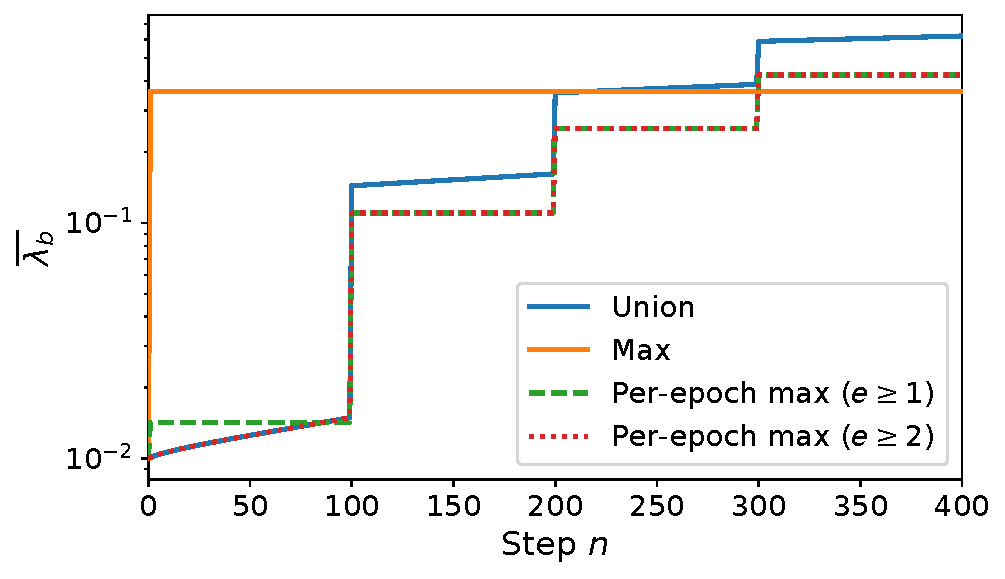
\includegraphics[width=\linewidth]{figures/union_vs_max_bound/dpsgd_4_epochs_100_batches_std_2.pdf}
        \subcaption{DP-SGD, $N=400,\ k=4,\ p=4,\ \sigma=2$}
    \end{subfigure}\hfill
    \begin{subfigure}[t]{0.45\linewidth}
        \centering
        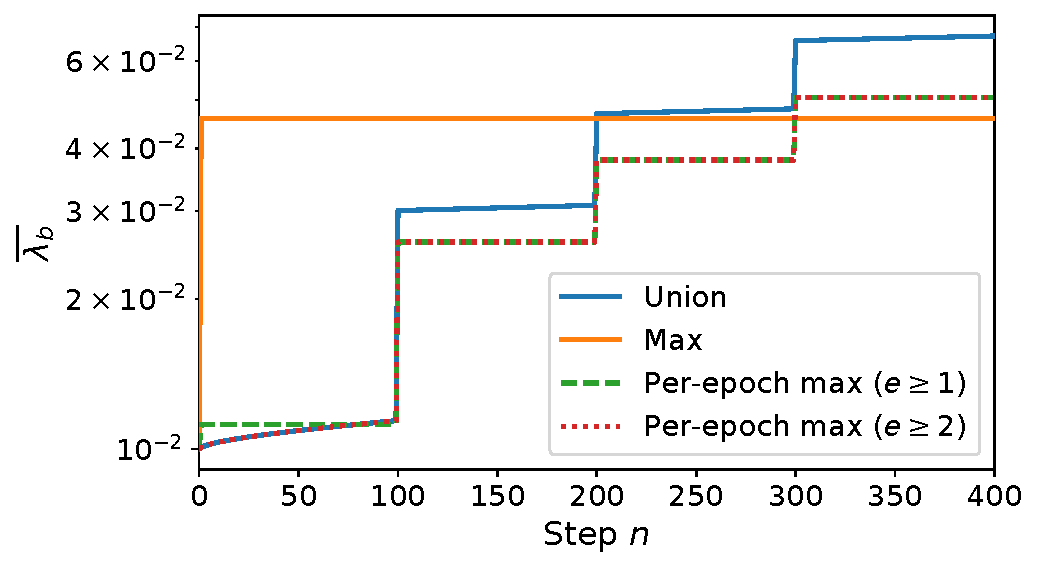
\includegraphics[width=\linewidth]{figures/union_vs_max_bound/dpsgd_4_epochs_100_batches_std_5.pdf}
        \subcaption{DP-SGD, $N=400,\ k=4,\ p=4,\ \sigma=5$}
    \end{subfigure}\hfill
    
    \begin{subfigure}[t]{0.45\linewidth}
        \centering
        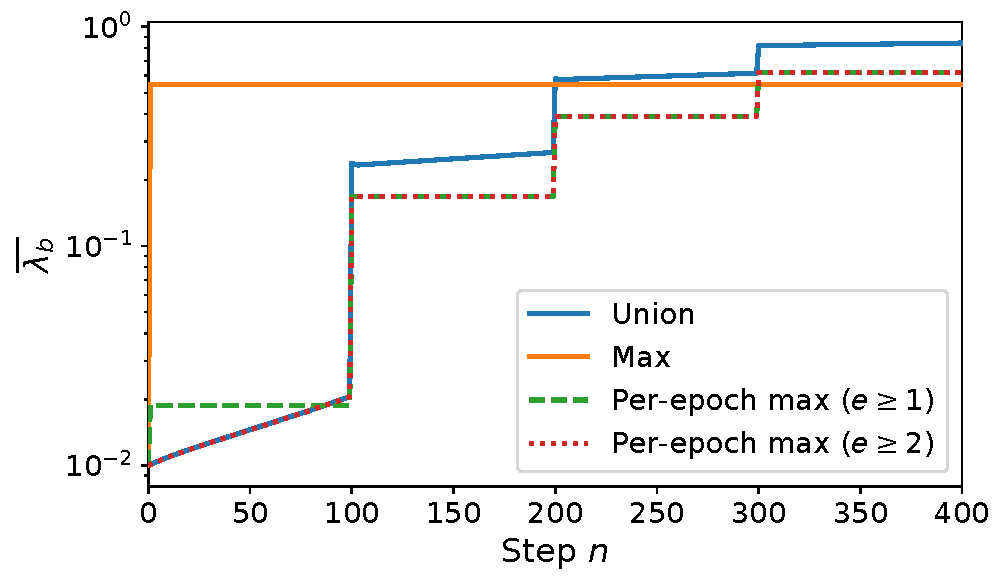
\includegraphics[width=\linewidth]{figures/union_vs_max_bound/bsr_4_epochs_100_batches_std_2.pdf}
        \subcaption{BSR, $N=400,\ k=4,\ p=4,\ \sigma=2$}
    \end{subfigure}\hfill
    \begin{subfigure}[t]{0.45\linewidth}
        \centering
        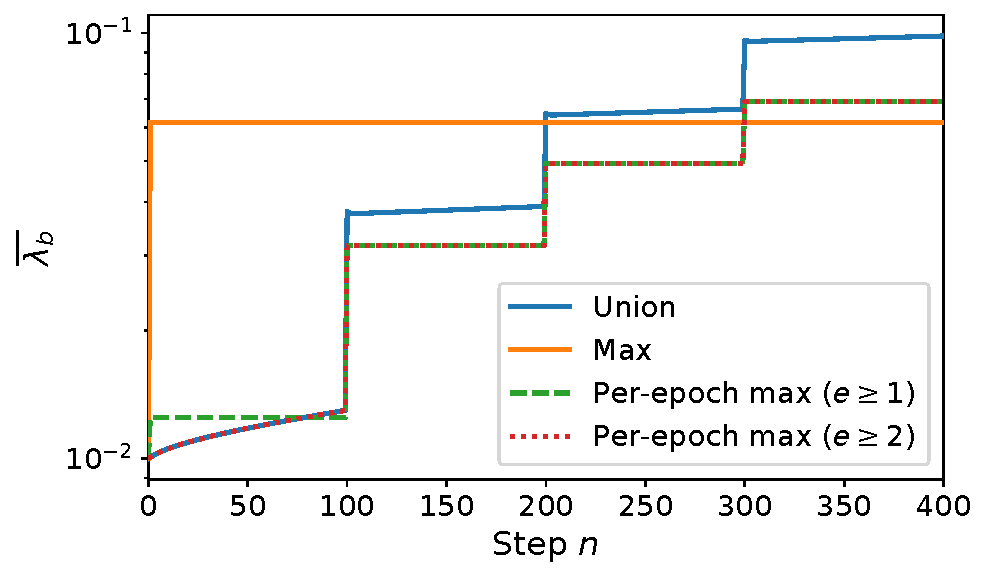
\includegraphics[width=\linewidth]{figures/union_vs_max_bound/bsr_4_epochs_100_batches_std_5.pdf}
        \subcaption{BSR, $N=400,\ k=4,\ p=4,\ \sigma=5$}
    \end{subfigure}\hfill
    \caption{Comparison of the largest mixture component's posterior probability $\overline{\lambda_b}$  (smaller is better)
    between different allocations of failure probability
    for different factorizations and noise multipliers $\sigma$ under $\delta_E = \SI{0.5e-5}{}$ and the ``remove'' relation.
    Using a union bound for the first epoch and a max bound for subsequent epochs (``Per-epoch max ($e \geq 2$)) performs best across most steps.
    Also using a max bound for the first epoch (``Per-epoch max ($e\geq 1$)) is only marginally better in the last few steps of the first epoch.
    Using a max bound across all steps (``Max'') is only marginally better in the last epoch and sacrifices the low subsampling rate $\overline{\lambda_b}$ of the first epoch's conditional composition dominating pairs.}
    \label{fig:experiment_union_vs_max_bound}
\end{figure}
\begin{figure}[h!]
    \centering

    \begin{subfigure}[t]{0.3\linewidth}
        \centering
        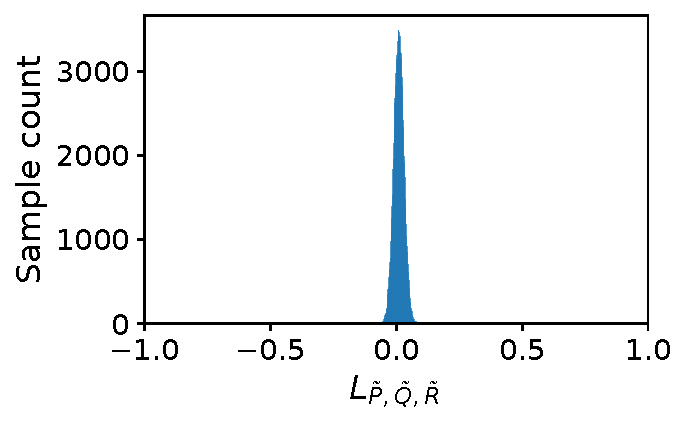
\includegraphics[width=\linewidth]{figures/posterior_jumps/dpsgd_4_epochs_100_batches_std_5.0_step_100.pdf}
        \subcaption{Step $100$}
    \end{subfigure}\hfill
    \begin{subfigure}[t]{0.3\linewidth}
        \centering
        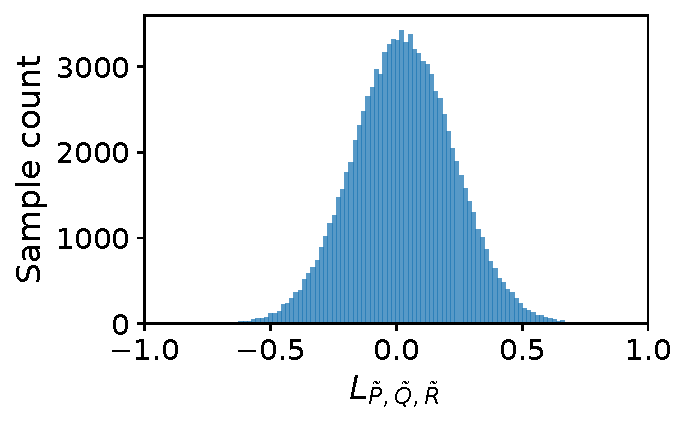
\includegraphics[width=\linewidth]{figures/posterior_jumps/dpsgd_4_epochs_100_batches_std_5.0_step_200.pdf}
        \subcaption{Step $200$}
    \end{subfigure}\hfill
    \begin{subfigure}[t]{0.3\linewidth}
        \centering
        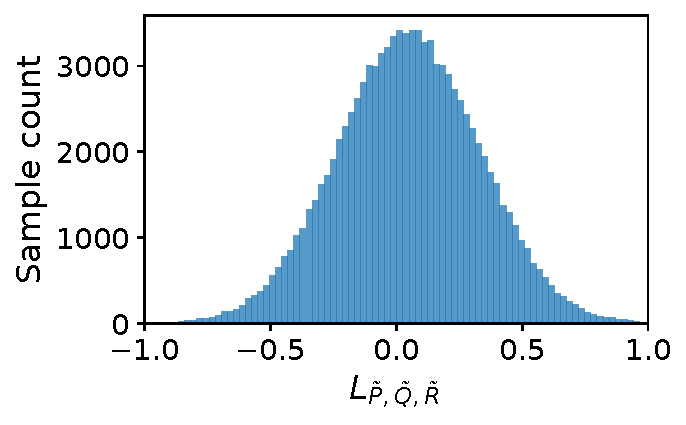
\includegraphics[width=\linewidth]{figures/posterior_jumps/dpsgd_4_epochs_100_batches_std_5.0_step_300.pdf}
        \subcaption{Step $300$}
    \end{subfigure}
    
    \begin{subfigure}[t]{0.3\linewidth}
        \centering
        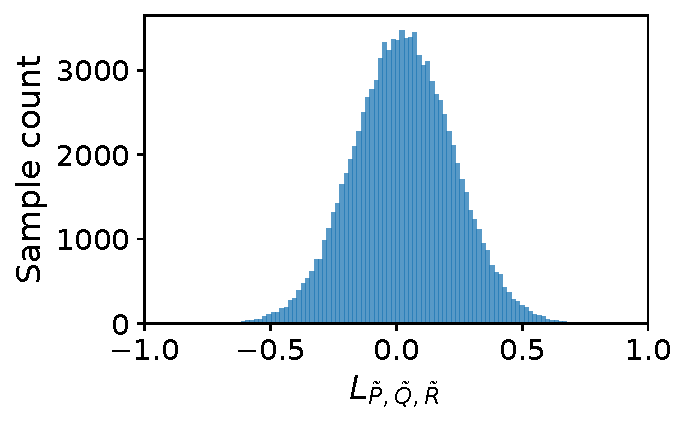
\includegraphics[width=\linewidth]{figures/posterior_jumps/dpsgd_4_epochs_100_batches_std_5.0_step_101.pdf}
        \subcaption{Step $101$}
    \end{subfigure}\hfill
    \begin{subfigure}[t]{0.3\linewidth}
        \centering
        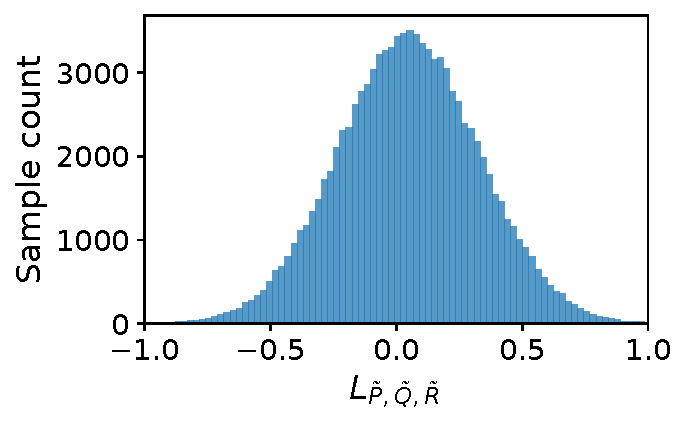
\includegraphics[width=\linewidth]{figures/posterior_jumps/dpsgd_4_epochs_100_batches_std_5.0_step_201.pdf}
        \subcaption{Step $201$}
    \end{subfigure}\hfill
    \begin{subfigure}[t]{0.3\linewidth}
        \centering
        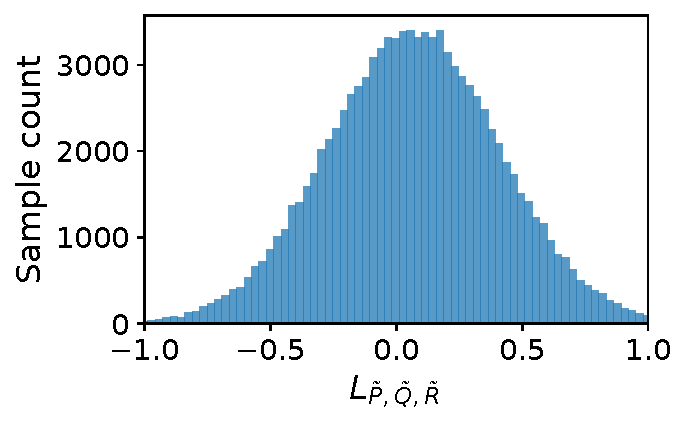
\includegraphics[width=\linewidth]{figures/posterior_jumps/dpsgd_4_epochs_100_batches_std_5.0_step_301.pdf}
        \subcaption{Step $301$}
    \end{subfigure}

    \caption{Sample histogram of the ternary privacy loss $L_{\tilde{P},\tilde{Q},\tilde{R}}$, whose lower tail is used to find reverse hazard upper bound $\overline{\lambda_b}$, shown at transitions between epochs.
    Samples are taken for DP-SGD with $k=4$ epochs, $b=100$ batches per epoch, and noise multiplier $\sigma=5$ for the ``remove'' relation.
    The histogram widens between epochs, which explains observed jumps in the reverse hazard bound.}
    \label{fig:posterior_jumps}
\end{figure}

\subsection{Remark on Jumps in Reverse Hazard}
At first, the jumps in our reverse hazard upper bound, which can be observed in both~\cref{fig:experiment_union_vs_max_bound} and~\cref{fig:experiment_variational_family} may seem abnormal or like an implementation error.
However, this is not the case. As an example, consider DP-SGD with $k$ epochs, $b$ batches per epoch, and $N = k \cdot b$ iterations overall. From the definition of our dominating pair in~\cref{lem:dominating_pair}, we know that the mixture means $\mm \in \sR^{k \cdot N}$ are simply
\begin{equation*}
    \mm = \begin{bmatrix}
        \eye_{b}\\
        \eye_{b}\\
        \cdots\\
        \eye_{b}
    \end{bmatrix},
\end{equation*}
i.e., a vertical stack of identity matrices, each with shape $b \times b$.
Consider an arbitrary step $n \in [N]$.
Recall from~\cref{algorithm:conditional_composition} that, to find our bound $\overline{\lambda_b}$ on the reverse hazard of the largest mixture component, we derive a lower tail bound on the ternary privacy loss $L_{\tilde{P}, \tilde{Q},\tilde{R}} = \log\left(\frac{\dd \tilde{P}}{\tilde{Q}}\right)(\vx)$ with $\vx \sim \tilde{R}$. Here, $\tilde{P}$ is a uniform mixture with means $\vmu_1, \dots, \vmu_{b-1} \in \{0,1\}^{n-1}$ taken from $\mm_{:, 1:n-1}$.
The distribution $\tilde{Q}$ is a single Gaussian with mean $\vmu_b \in \{0,1\}^{n-1}$.
In epoch $e = (n \mod b) + 1$, the single mean $\vmu_b$ of $\tilde{Q}$ has $\max\{e-1, 0\}$ non-zero entries.
Similarly, each mean $\vmu_j$ of $\tilde{P}$ has either $e$ or $\max\{e-1,0\}$ non-zero entries in distinct dimensions.
Thus, the pairwise distance between $\vmu_i$ and any $\vmu_j$ fulfills
\begin{equation*}
    ||\vmu_j - \vmu_i||_2 \in \{\sqrt{2e-1}, \sqrt{2e-2}\}.
\end{equation*}
Thus, the privacy loss increases from epoch to epoch.
In~\cref{fig:posterior_jumps}, we empirically verify this effect by taking $\SI{100000}{}$ samples from $L_{\tilde{P}, \tilde{Q}, \tilde{R}}$
for DP-SGD at the end and start of each epoch for $k=4$, $b=100$, $\sigma=5$.
We observe that the sample histogram of the privacy loss distribution significantly widens when transitioning from one epoch to the next.


\clearpage

\iffalse
\section{Asymptotic Analysis of the Variational Privacy Loss Bounds}

While~\cref{thm:remove_tail_bound} and~\cref{thm:add_tail_bound} provide an exact way to compute tail bounds using the Gaussian CDF, they do not explicitly show how the tail bounds scale with the means $\mm_1,\dots, \mm_b \in \sR^{N}$ and the noise multiplier $\sigma \in \sR_+$ of the matrix mechanism's overall dominating pair from~\cref{lem:dominating_pair}.
In particular, it does not show how the failure probability $\beta_i$ for each step $n \in N$ and each mixture component $i \in [b]$ (recall~\cref{algorithm:conditional_composition})
scales with the prefixes $\vmu_1 = \mm_{1,:n-1}, \dots, \vmu_b = \mm_{b,:n-1}$
that are used to construct per-iteration dominating pair $P^{(n)},Q^{(n)}$.


To analyze the asymptotic behavior, we apply standard Gaussian concentration inequalities to the previously derived bounds. For simplicity, we focus on the ``add'' case (a similar result could be shown for the remove case by taking the maximum over all mixture components).
\begin{proposition}\label{prop:asymptotic_bound}
    Let $\underline{L_i}(\vx) \sim \mathcal{N}(\nu, \xi)$ be the variational privacy loss lower bound derived in \cref{thm:add_tail_bound}. For any threshold $\tau < \nu$, the tail probability is bounded by:
    \begin{equation}
        \Pr[L_i(\vx) \leq \tau] \leq \exp\left( - \frac{(\nu - \tau)^2}{2\xi^2} \right),
    \end{equation}
    with
    \begin{align*}
        \nu &= \frac{1}{2\sigma^2} \left( \|\vmu_i\|_2^2 - \mathbb{E}_{j \sim \psi^{(k)}}[\|\vmu_j\|_2^2] \right) - \mathrm{KL}(\psi \mid\mid \pi), \\
        \xi &= \frac{1}{\sigma} \| \vmu_i - \mathbb{E}_{j \sim \psi}[\vmu_j] \|_2.
    \end{align*}
\end{proposition}

\begin{proof}
    The random variable $L_i(\vx)$ follows a normal distribution with mean $\nu$ and standard deviation $\xi$. We standardize this variable to $Z = \frac{L_i(\vx) - \nu}{\xi}$, which follows $\mathcal{N}(0, 1)$.
    The event $L_i(\vx) \leq \tau$ is equivalent to $Z \leq \frac{\tau - \nu}{\xi}$. Defining $t = \frac{\nu - \tau}{\xi}$, the condition $\tau < \nu$ implies $t > 0$.
    Applying the standard Gaussian concentration inequality $\Pr[Z \leq -t] \leq e^{-t^2/2}$ and substituting $t$ yields the result.
\end{proof}

To interpret this bound, we analyze the case of a uniform variational distribution $\psi$.
There, the parameters simplify to $\nu = \frac{1}{\sigma^2} (\|\vmu_i\|_2^2 - \overline{\|\vmu\|_2^2})$ and $\xi = \frac{1}{\sigma} \|\vmu_i - \bar{\vmu}\|_2$,
with averages $\overline{\|\vmu\|_2^2} = \frac{1}{i-1} \sum_{j=1}^{i-1} ||\vmu_j||_2^2$ and  $\bar{\vmu} = \frac{1}{i-1} \sum_{j=1}^{i-1} \vmu_j$.
Substituting these into \cref{prop:asymptotic_bound} with $\tau=0$ yields an exponent of the form:
\begin{equation}
    \frac{\nu^2}{2\xi^2} = \frac{1}{8\sigma^2} \cdot \underbrace{\frac{ \left( \|\vmu_i\|_2^2 - \overline{\|\vmu\|_2^2} \right)^2 }{ \|\vmu_i - \bar{\vmu}\|_2^2 }}.
\end{equation}
Consequently, ...

\clearpage


\fi


\section{Choice of Variational Family}\label{appendix:choice_of_variational_family}
Recall from~\cref{algorithm:conditional_composition} that we need to find a lower tail bound on the ternary privacy loss  random variable $L_{\tilde{P}, \tilde{Q}, \tilde{R}}$,
which is defined as $L_i(\vx)$ with $L_i(\vx) = \log\left(\frac{\dd \tilde{P}}{\dd \tilde{Q}}\right)(\vx)$ and $\vx \sim \tilde{R}$,
where $\tilde{P}$ is a uniform Gaussian mixture with means $\vmu_1,\dots,\vmu_{i-1}$,
$\tilde{Q}$ is a single Gaussian with mean $\vmu_i$,
and $\tilde{R}$ is either:
\begin{itemize}
    \item $\sum_{k=i}^{b} \mathcal{N}(\mmu_k, \sigma^2 \eye_{n-1}) \cdot \frac{1}{b}$ (``remove'' case),
    \item or $\mathcal{N}(\vzero, \sigma^2 \eye_{n-1})$ (``add'' case), which is equivalent to the trivial mixture
    $\sum_{k=i}^{b} \mathcal{N}(\vzero, \sigma^2 \eye_{n-1}) \cdot \frac{1}{b}$.
\end{itemize}
Let $\vrho_k \in \sR^{n-1}$ denote an arbitrary component mean of $\tilde{R}$ (either $\vmu_k$ or the all-zeros vector $\vzero$).
From~\cref{lemma:variational_distribution_general,thm:remove_tail_bound,thm:add_tail_bound}, we know that the tail probability conditioned on component $k$ is upper-bounded via
\begin{equation}\label{eq:single_component_tail_bound}
    \Pr_{\vx \sim \mathcal{N}(\vrho_k, \sigma^2 \eye)}[L_i(\vx) \leq \tau] \leq \Phi\left( \frac{\tau - \nu_k}{\xi_k} \right)
\end{equation}
with scalar mean $\nu_k \in \sR$ and scalar standard deviation $\xi_k \in \sR_+$
with
\begin{align}
    \nu_k &= \frac{1}{\sigma^2} \vmu_k^T (\mathbb{E}_{j \sim \psi^{(k)}}[\vmu_j] - \vmu_i) + \frac{1}{2\sigma^2} \left( \|\vmu_i\|_2^2 - \mathbb{E}_{j \sim \psi^{(k)}}[\|\vmu_j\|_2^2] \right) - \mathrm{KL}(\psi^{(k)} \mid\mid \pi),
    \label{eq:variational_per_component_mean}
    \\
    \xi_k &= \frac{1}{\sigma} \| \vmu_i - \mathbb{E}_{j \sim \psi^{(k)}}[\vmu_j] \|_2,
    \label{eq:variational_per_component_std}
    \\
    \pi &= \mathrm{Uniform}(\{1,\dots,i-1\}),
\end{align}
for any variational distribution $\psi^{(k)}$ over mixture indices $\{1,\dots, i-1\}$.
Therefore, we can define an entire variational family $\Psi^{(k)}$ and choose a $\psi^{(k)} \in \Psi^{(k)}$ that leads to the tightest tail bound.

In principle, we could let $\Psi^{(k)}$ be the set of all distributions supported on $\{1,\dots, i-1\}$ and explicitly optimize $\psi^{(k)}$ (e.g., via gradient descent, which would be an interesting direction for future work).
However, for $k \in \sN$ epochs and $b \in \sN$ batches per epoch and thus $N = k \cdot b$, we would need to solve
$N \cdot b^2$ such optimization problems (one for each step $n$, each privacy loss $L_i$ with $i \in [b]$, and  each component $k \in [b]$ of $\tilde{R})$. 
We therefore consider the following heuristically chosen variational families instead:

\subsection{Option 1: Maximizing the expectation based on KL divergence}
A heuristic for tightening the bound in~\cref{eq:single_component_tail_bound}
is by maximizing the mean $\nu_k$.
In turn, a heuristic for doing so is to eliminate the  KL-divergence term in~\cref{eq:variational_per_component_mean}
by letting
\begin{equation*}
    \psi^{(k)} = \pi = \mathrm{Uniform}(\{1,\dots, i-1\}.
\end{equation*}
This corresponds to taking the geometric mean of privacy losses, which we already used in deriving our R\'enyi divergence bound from~\cref{lem:remove-renyi-bound}.

\subsection{Option 2: Maximizing the expectation based on component distance}
Another heuristic for maximizing the mean is to apply quadratic expansion, i.e., 
\begin{equation*}
    \nu_k = - \frac{1}{2 \sigma^2} \mathbb{E}_{j \sim \psi^{(k)}}\left[||\vrho_k - \vmu_j||_2^2\right]
    + \frac{||\vrho_k - \vmu_i||_2^2}{2\sigma^2} - \mathrm{KL}(\psi^{(k)} || \pi),
\end{equation*}
and notice that the second term does not depend on variational distribution $\psi^{(k)}$.
Instead of minimizing the KL-divergence, we could instead define $\psi^{(k)}$ to minimize the distance in the first term, i.e., $\psi^{(k)}(z=j) = 1 \iff j = \mathrm{argmin} ||\rho_k - \vmu_j||_2^2$.
To smoothly interpolate between this solution and minimization of the KL divergence, we can define
the variational family as
$\Psi^{(k)} = \{\psi(t, \vrho_k, (\vmu_1,\dots,\vmu_{i-1}\}) \mid t \in T\}$ with
\begin{equation*}
    \psi(t, \vrho_k, (\vmu_1,\dots,\vmu_{i-1})\}
    = \mathrm{softmax}\left( \left\{- \frac{||\vrho_k - \vmu_j||_2^2}{t } \middle| 1 \leq j < i\right\} \right)
\end{equation*}
for some fixed set of non-negative temperatures $T \subset \sR_+$.

\subsection{Option 3: Minimizing the standard deviation based on component distance}
Another heuristic for tightening the tail bound in~\cref{eq:single_component_tail_bound}
is by minimizing the standard deviation $\nu_k$, which makes the argument of Gaussian CDF $\Phi$ smaller for any $\tau \leq \nu_k$, i.e., any tail probability smaller than $0.5$.
Analogous to the previous approach, we can define
$\Psi^{(k)} = \{\psi(t, \vmu_i, (\vmu_1,\dots,\vmu_{i-1})\} \mid t \in T\}$ with
\begin{equation*}
    \psi(t, \vmu_i, (\vmu_1,\dots,\vmu_{i-1})\}
    = \mathrm{softmax}\left( \left\{- \frac{||\vmu_i - \vmu_j||_2^2}{t } \middle| 1 \leq j < i\right\} \right)
\end{equation*}
for some fixed set of non-negative temperatures $T \subset \sR_+$.
Notice that, unlike the previous approach, this variational family is independent of the component mean $\vrho_k$, i.e.,
we use the same variational family across all components of $\tilde{R}$.

\subsection{Our choice.}
In our experiments, we opt for Option 3, since it only requires evaluation of a linear number of distances $||\vmu_i - \vmu_j||$,
and this computational cost is shared across all $K$ components of our tail bound.
We additionally include $\tau = \infty$, which corresponds to the KL-minimizing uniform distribution from Option 1.
For our experiments, we specifically use temperatures $T = \{\infty\} \cup \{10^{-1}, 10^{-0.5}, 1, 10^{0.5}, 10^{1}\}$, which we found to improve tightness of our accountant compared to Option 1 ($T = \{\infty\}$) alone, i.e., the geometric mean.
Furthermore, we empirically did not find Option 2 to offer any increased tightness.
\cref{fig:experiment_variational_family} demonstrates this through an empirical comparison across different matrix factorizations and noise levels in the multi-epoch setting.

\begin{figure}[h]
    \centering

    \begin{subfigure}[t]{0.45\linewidth}
        \centering
        
\includegraphics[width=\linewidth]{figures/variational_family/bsr_4_epochs_100_batches_std_2.pdf}
        \subcaption{BSR, $N=400,\ k=4,\ p=4,\ \sigma=2$}
    \end{subfigure}\hfill
    \begin{subfigure}[t]{0.45\linewidth}
        \centering
        
\includegraphics[width=\linewidth]{figures/variational_family/bsr_4_epochs_100_batches_std_5.pdf}
        \subcaption{BSR, $N=400,\ k=4,\ p=4,\ \sigma=5$}
    \end{subfigure}\hfill
    
    \begin{subfigure}[t]{0.45\linewidth}
        \centering
        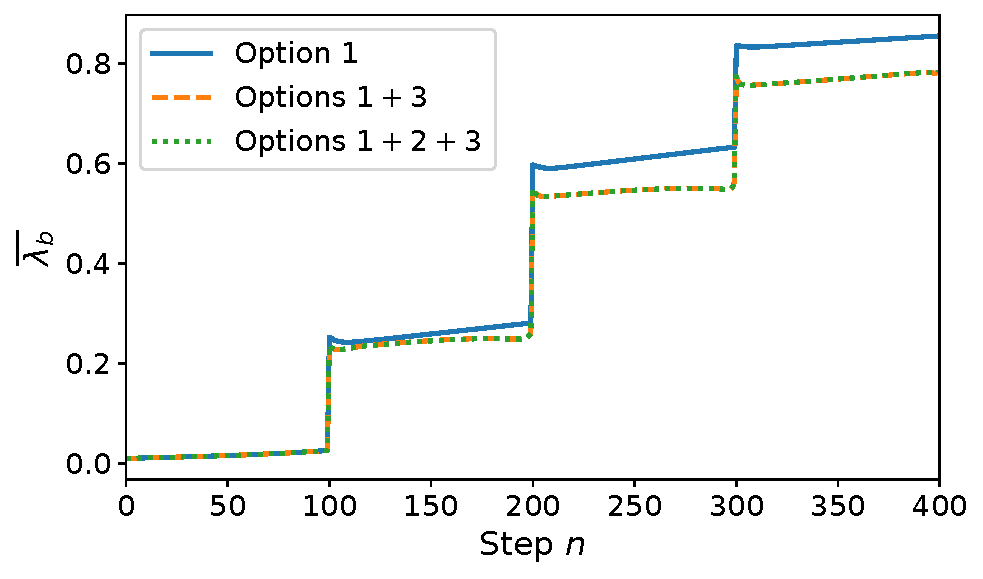
\includegraphics[width=\linewidth]{figures/variational_family/bisr_4_epochs_100_batches_std_2.pdf}
        \subcaption{BISR, $N=400,\ k=4,\ p=4,\ \sigma=2$}
    \end{subfigure}\hfill
    \begin{subfigure}[t]{0.45\linewidth}
        \centering
        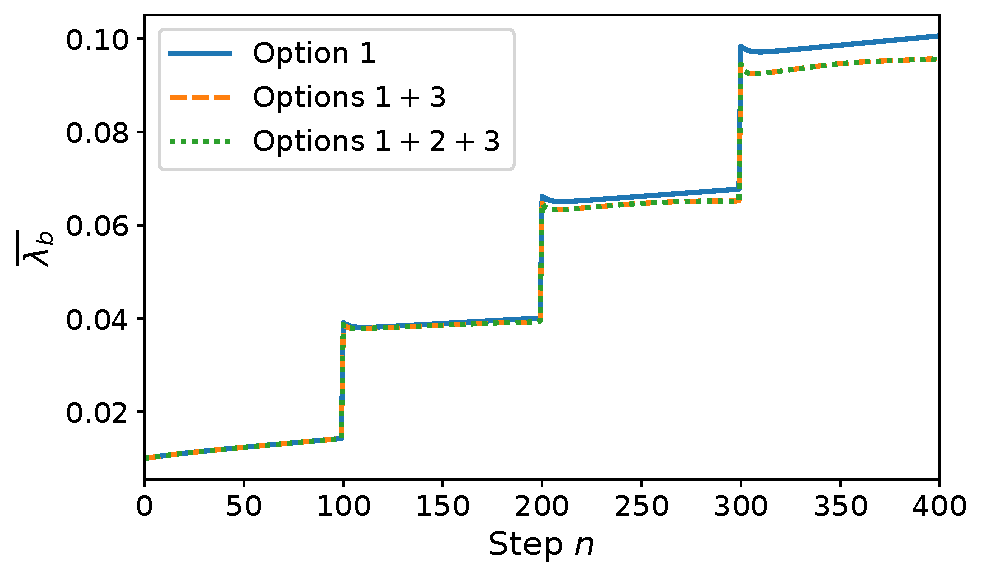
\includegraphics[width=\linewidth]{figures/variational_family/bisr_4_epochs_100_batches_std_5.pdf}
        \subcaption{BISR, $N=400,\ k=4,\ p=4,\ \sigma=5$}
    \end{subfigure}\hfill
    \caption{Comparison of the largest mixture component's posterior probability $\overline{\lambda_b}$  (smaller is better)
    between variational families 
    for different factorizations and noise multipliers $\sigma$ under $\delta_E = 10^{-5}$ and the ``remove'' relation.
    In later epochs, minimizing variance of the tail bound (``Options 1+3'') improves upon only taking the geometric mean 
    via a uniform distribution (``Option 1'').
    The effect is more pronounced in settings where  the noise multiplier is small and sensitivity is large ($\sigma=2$, BISR),
    compared to settings where the noise multiplier is large and the overall sensitivity is small ($\sigma=5$, BSR).
    Maximizing the mean (``Option 2'') does not further improve the posterior bound.
    }
    \label{fig:experiment_variational_family}
\end{figure}

\subsection{Overall Computational Cost of Tail Bounds}
In each step $n \in [N]$ and for each component $i \in [b]$, 
the cost of deriving the tail bound $\tau_i$ in~\cref{algorithm:conditional_composition} is dominated by computing distances $\|\boldsymbol{\mu}_i - \boldsymbol{\mu}_j\|^2$, each of which has a cost of $\mathcal{O}(n)$. A na\"ive implementation of re-computing these distances for vectors in $\mathbb{R}^n$ at every step and for each component leads to an overall complexity  of $\mathcal{O}(N^2 b^2)$.
We use this na\"ive approach in the implementation provided with the supplementary material.

However, to scale to larger $N$, one could in principle reduce the overall cost to $\mathcal{O}(N b^2)$ using incremental updates. By maintaining the Gram matrix of the mixture means $\vmu_1,\dots,\vmu_b$ starting from step $n=1$, one can exploit the prefix structure of the means: the inner products for step $n$ are simply those of step $n-1$ plus the product of the current batch contributions. This would allow for constant-time distance evaluation at each step after a $\mathcal{O}(b^2)$ update.

\clearpage

\section{Add and Remove Direction Dominating Pairs}\label{appendix:add_remove_flip}
Recall that we assume the following dominating pair:
\fulldominatingpair*
That is:
\begin{itemize}[nosep]
    \item In the ``remove'' case, $P$ is a Gaussian mixture and $Q$ is a single multivariate Gaussian.
    \item In the ``add'' case $P$ is a single Gaussian and $Q$ is a Gaussian mixture.
\end{itemize}
In the original Lemma 3.2 of~\cite{choquette2024near}, the directions are reversed. However, this appears to be a typing error.
Their proof for the ``add'' case actually argues correctly that the first argument of the hockey-stick divergence should be a zero-mean  Gaussian and the second argument should be a Gaussian mixture (note that in their proof $\vz$ is a zero-mean Gaussian):
``We give the proof for the \underline{add adjacency} [...]
Because each user is assigned to their batch independently, we can assume without loss of generality that contributions from all users other than the differing user are always $0$. In more detail, by post-processing, we can assume that we release the contributions to the input matrix of all examples except the differing user's. Let $\vx$ be these contributions, and $\vx'$ be $\vx$ plus the contribution of the differing user. Then distinguishing $\mC \vx + \vz$ and $\mC \vx' + \vz$ is equivalent to \underline{distinguishing $\vz$ and $\mC (\vx' - \vx) + \vz$} [ ...]``.

Further note that the same pattern of $P$ being a mixture under ``remove'' and $Q$ being a mixture under ``add'' arises in various other subsampling schemes, such as Poisson subsampling or subsampling without replacement (see, e.g., Theorem 11 in~\cite{zhu2022optimal}).


\end{document}

% This document was modified from the file originally made available by
% Pat Langley and Andrea Danyluk for ICML-2K. This version was created
% by Iain Murray in 2018, and modified by Alexandre Bouchard in
% 2019 and 2021 and by Csaba Szepesvari, Gang Niu and Sivan Sabato in 2022.
% Modified again in 2023 and 2024 by Sivan Sabato and Jonathan Scarlett.
% Previous contributors include Dan Roy, Lise Getoor and Tobias
% Scheffer, which was slightly modified from the 2010 version by
% Thorsten Joachims & Johannes Fuernkranz, slightly modified from the
% 2009 version by Kiri Wagstaff and Sam Roweis's 2008 version, which is
% slightly modified from Prasad Tadepalli's 2007 version which is a
% lightly changed version of the previous year's version by Andrew
% Moore, which was in turn edited from those of Kristian Kersting and
% Codrina Lauth. Alex Smola contributed to the algorithmic style files.
